% !TeX root = ../../tesi.tex

\subsection{Site 1: Volume Estimation}
The volume-estimation branch at Site~1 was developed through several increasingly refined workflows. A first baseline estimated volume by computing a convex hull directly from the points contained within each detected bounding box. However, this bounding-box-only approximation was not sufficiently accurate, because the selected region also included non-dough elements that biased the reconstructed geometry. Subsequent variants therefore introduced an explicit segmentation stage before volumetric reconstruction. SAM \cite{kirillov_segment_2023} was first explored as a foreground-segmentation tool and produced very accurate masks, but its computational cost proved too high for the intended workflow, whose long-term goal is deployment on edge devices. The final implementation therefore relies on a more efficient pipeline based on color clustering, refined through depth-based background subtraction and followed by axis-based 3D completion.\cite{labby_thesis_repo_2026}

\subsubsection{Detection Filtering}
Before volumetric processing, the detections are filtered so as to retain only the most reliable samples. In particular, a dedicated preprocessing stage builds a filtered detection cache by keeping only images containing a single valid dough-ball detection inside a predefined ROI polygon. This step reduces ambiguities caused by multiple simultaneous objects, spurious detections near the borders of the acquisition area, or colliding dough balls, all of which can be problematic for the subsequent volume-estimation stage.

This filtering stage was introduced because the main aim of this part of the thesis is to analyze the consistency of the volume-estimation algorithms on a well-defined set of samples, rather than to evaluate the robustness of the detector under crowded or ambiguous conditions. According to the nominal operating conditions of the line, multiple dough balls should not be present simultaneously on the output table; frames exhibiting such cases were therefore treated as outliers and excluded from the analysis.
\newpage

\subsubsection{Reference Table Modelling}
The supporting table is modelled separately from a set of empty-scene acquisitions. These depth images are aggregated through a robust median operation in order to produce a reference depth background for the table. The resulting model is stored as a numerical depth map for subsequent computations and can also be exported as a point cloud or mesh for debugging and visualization purposes, as shown in Figure~\ref{fig:table_model}.\cite{labby_thesis_repo_2026} This reference surface is later used both to remove the support contribution from the dough point cloud and to define the geometric relation between the visible dough region and the table plane.

\begin{figure}[!htbp]
    \centering
    \begin{subfigure}[b]{0.48\textwidth}
        \centering
        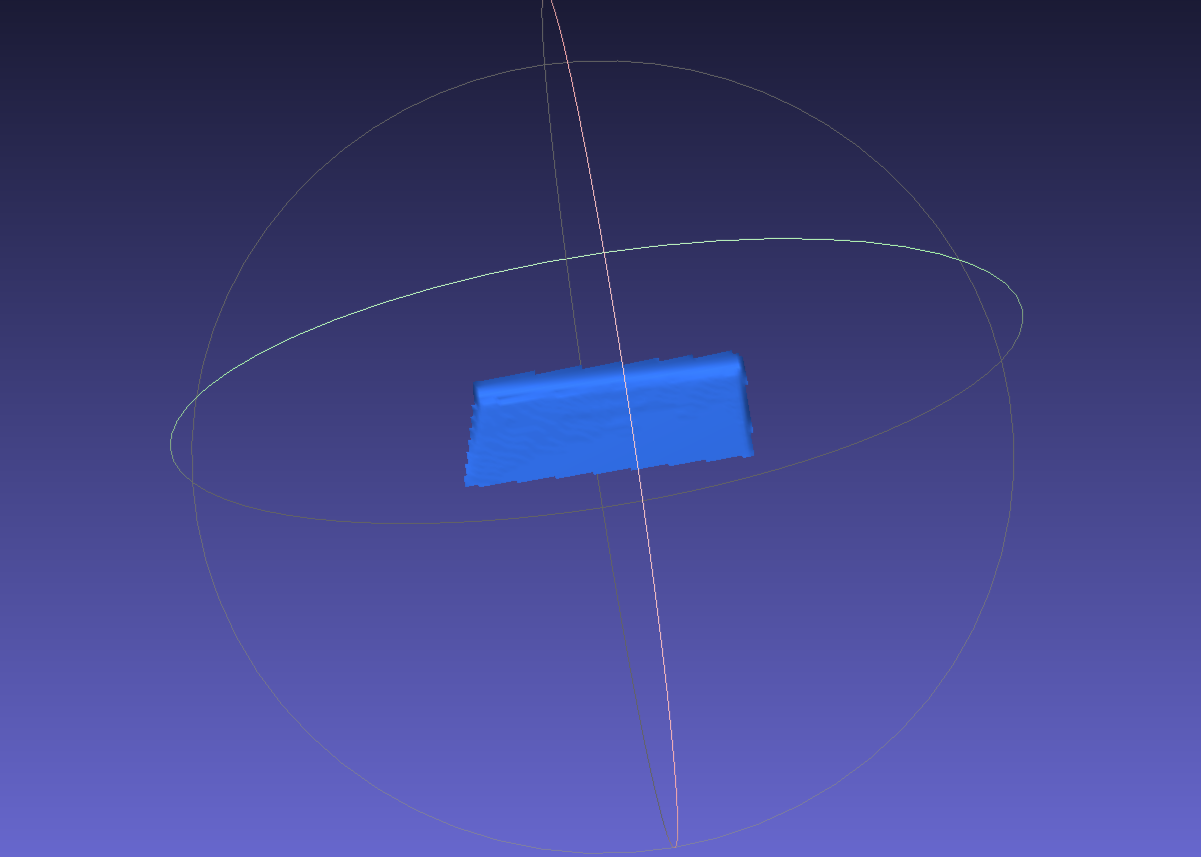
\includegraphics[width=\linewidth]{images/Useful-photos/Screenshots/BG_table.png}
        \caption{Front view}
    \end{subfigure}
    \hfill
    \begin{subfigure}[b]{0.48\textwidth}
        \centering
        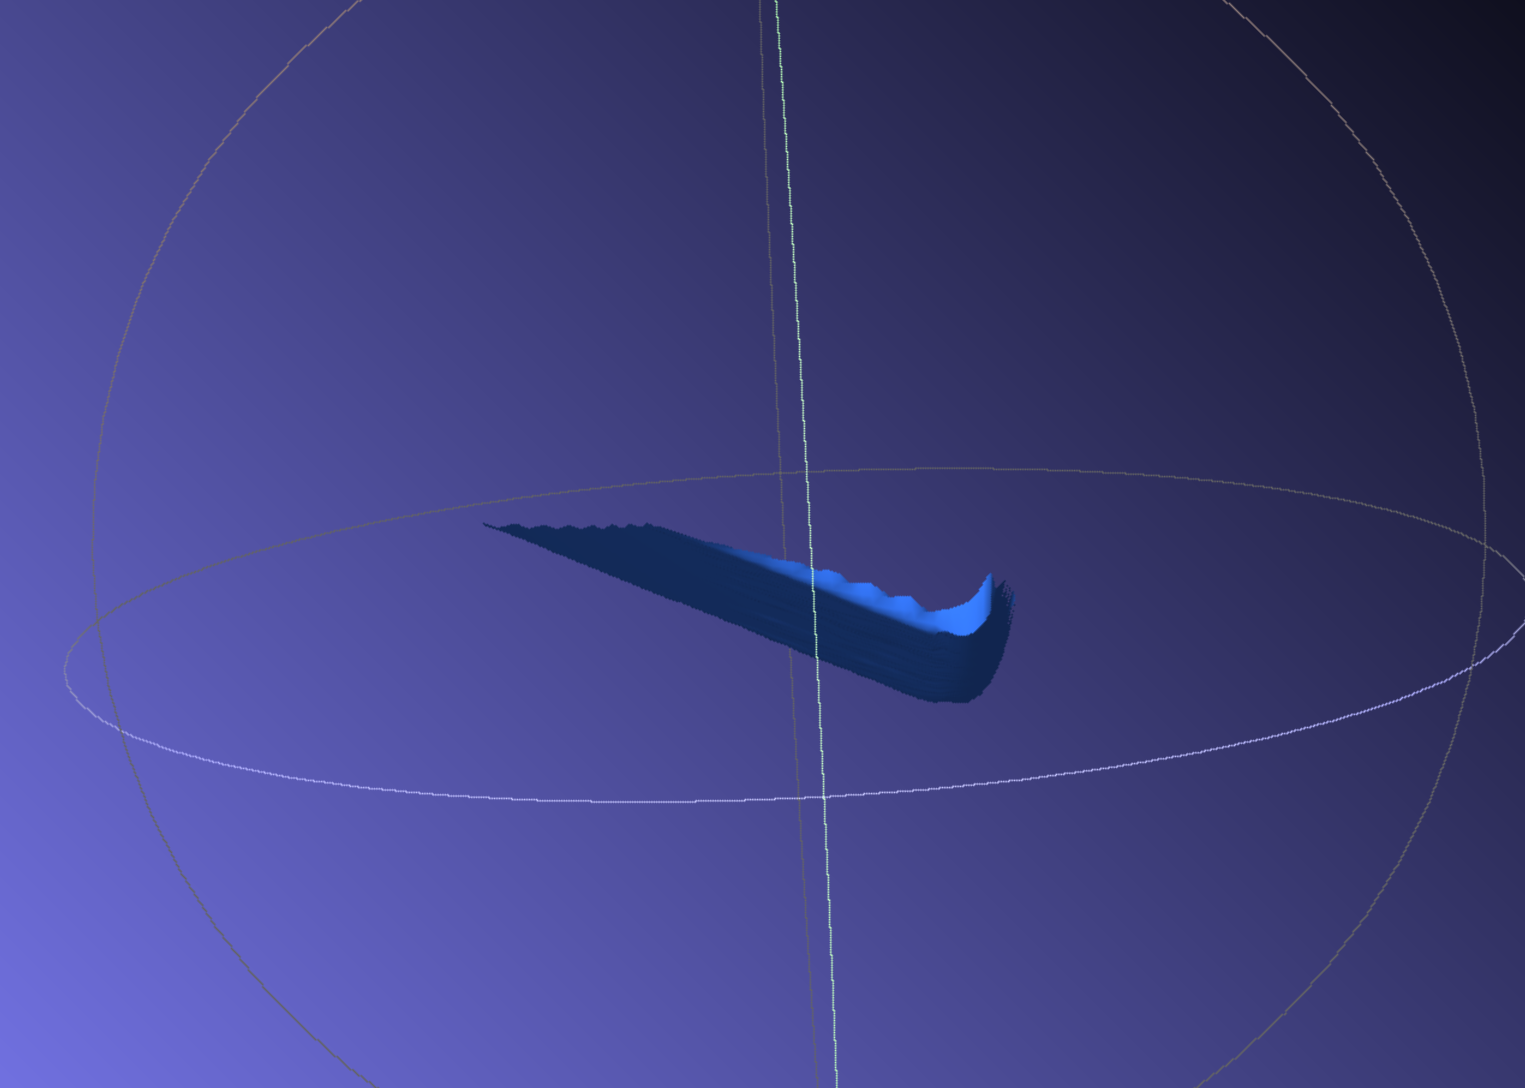
\includegraphics[width=\linewidth]{images/Useful-photos/Screenshots/BG_table2.png}
        \caption{Side view}
    \end{subfigure}
    \caption{Reference table model reconstructed from empty-scene depth acquisitions.}
    \label{fig:table_model}
\end{figure}

\subsubsection{Foreground Extraction and Point-Cloud Generation}
Once a dough-ball detection has been selected, the corresponding RGB bounding box is associated with the aligned depth image through the Kinect calibration and reprojection pipeline. Because the RGB and depth streams of the Azure Kinect have different intrinsic parameters, extrinsic relationships, and fields of view, a dedicated reprojection and alignment stage was implemented using the calibration data provided by the Azure Kinect SDK and accessed in Python through the \textit{pyKinectAzure} interface.\cite{microsoft_azure-kinect-sensor-sdk_2026,gorordo_fernandez_pykinectazure_2026} This stage makes it possible to map the RGB detections onto the corresponding depth coordinates and therefore to associate each RGB bounding box with the correct 3D measurements.

\begin{figure}[h]
    \centering
    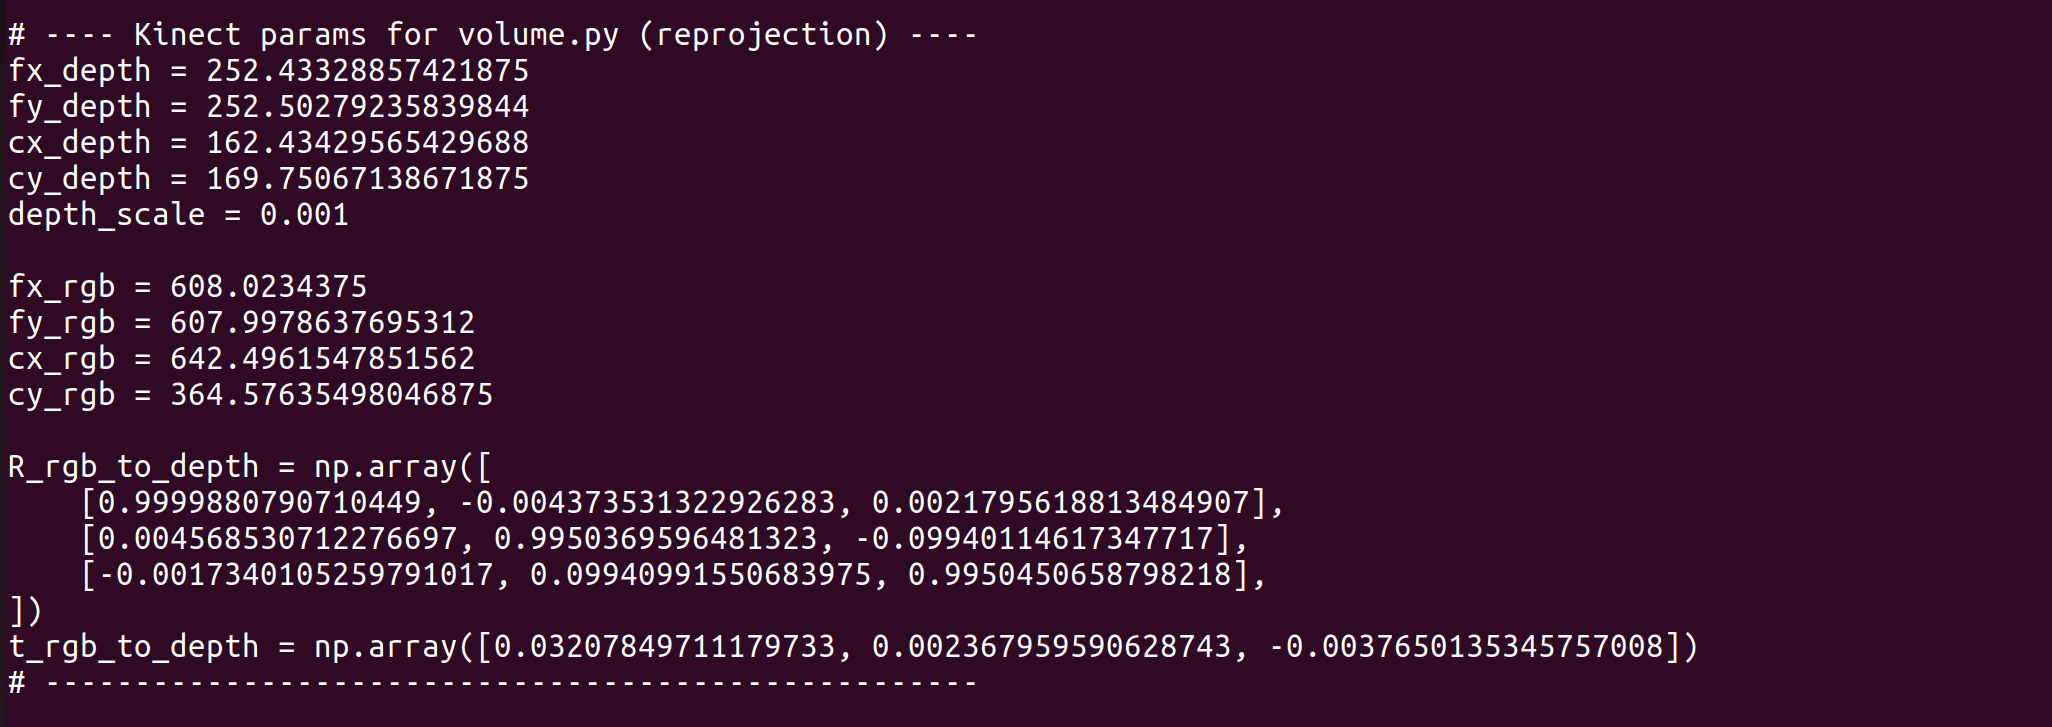
\includegraphics[width=0.80\textwidth]{images/Reprojection_param.png}
    \caption{Kinect reprojection parameters. The figure shows the RGB and depth intrinsic parameters, as well as the extrinsic transformation between the two sensors, which are used to align the RGB detections with the depth data.}
    \label{fig:reprojection_parameters}
\end{figure}

The local 3D point cloud is then obtained from the aligned depth pixels by means of the standard pinhole camera model:

\begin{equation}
X = \frac{(u - c_x) \cdot Z}{f_x}, \quad
Y = \frac{(v - c_y) \cdot Z}{f_y}, \quad
Z = D(u,v)
\end{equation}

where $(u,v)$ are the pixel coordinates, $D(u,v)$ is the depth value, $(c_x, c_y)$ are the principal-point coordinates, and $f_x$ and $f_y$ are the focal lengths expressed in pixel units.
\\
The implementation supports different segmentation modes, namely \texttt{sam}, \texttt{bbox}, and \texttt{color}.\cite{labby_thesis_repo_2026} These modes are configurable through the experiment configuration file, whereas the workflow adopted for the main experiments initializes the foreground in \texttt{color} mode and then refines it in depth (\texttt{color\_then\_depth}). More specifically, a central rectangular seed (shown in yellow in Figure~\ref{fig:color_segmentation}) is first derived from each detection, and the clustering stage can also be extended by a configurable percentage beyond the predicted bounding box so as to remain robust even when the detector localization is not perfectly tight. The color-based stage suppresses the blue background, constrains the admissible lightness range, optionally performs adaptive clustering in the \textsc{Lab} color space, and can recover dark dough regions that would otherwise be missed by a purely brightness-based filter.\cite{labby_thesis_repo_2026}

\begin{figure}[H]
    \centering
    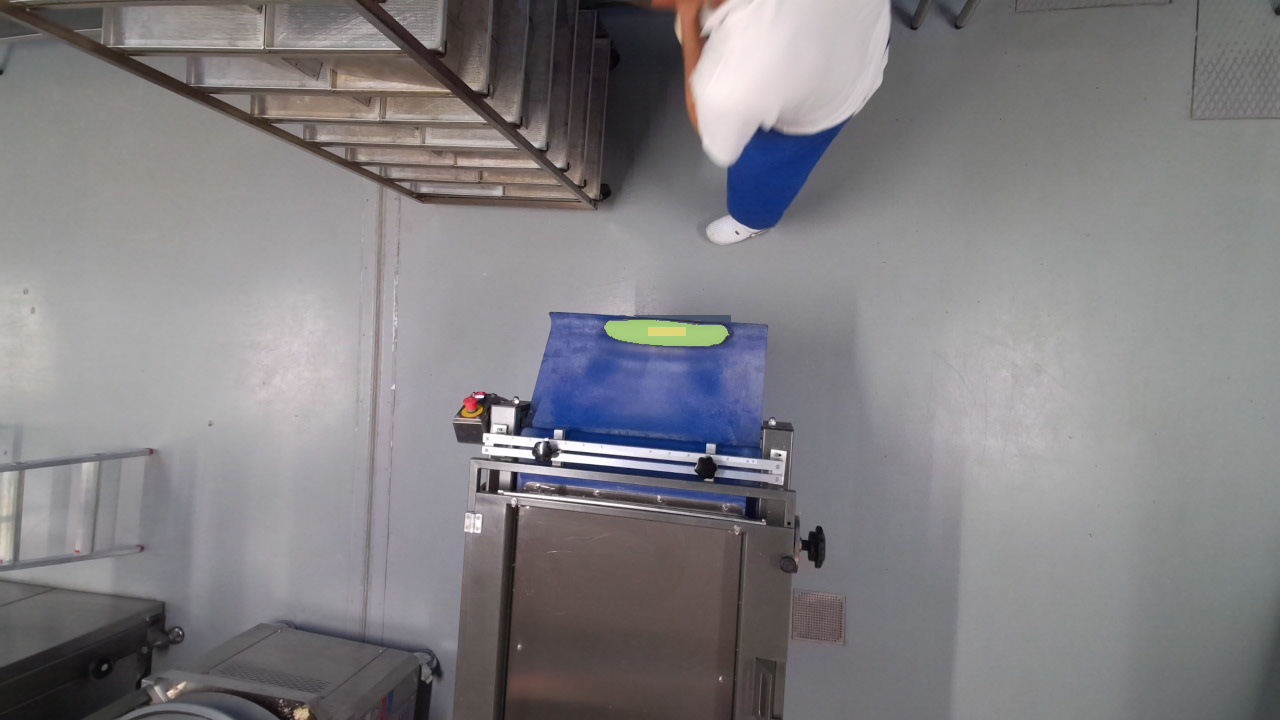
\includegraphics[width=0.70\textwidth]{images/Useful-photos/color_segmentation.png}
    \caption{Example of the color-based segmentation stage. The dough point cloud is shown in green, filtered points are highlighted in red, the seed rectangle is shown in yellow, and the background region excluded by clustering is shown in blue.}
    \label{fig:color_segmentation}
\end{figure}

In an earlier version of the workflow, this clustering step was not yet present; it was introduced later because it produced a cleaner foreground estimate before depth refinement. The resulting mask is then projected onto the depth data and further refined through background subtraction against the precomputed table model, with additional morphological filtering to improve spatial coherence.\cite{labby_thesis_repo_2026} A practical difficulty in this stage is that the depth measurements near the border of the table, especially along its final curved portion, may exhibit singular or unstable values that make the support surface harder to filter correctly. In this respect, the two refinement stages complement each other: color clustering helps suppress unstable depth regions near the table border before they enter the volumetric estimation, whereas background subtraction removes regions that may be chromatically similar to the dough but are not geometrically consistent with the support model. This issue is also mitigated by combining an adaptive background-subtraction threshold with the distance from the reference table surface. These morphological operations remove points in the point cloud that intersect, penetrate the table model, or are closer than a certain threshold to the background, thereby enforcing a geometrically consistent foreground prior to volumetric reconstruction.

\begin{figure}[H]
    \centering
    \begin{subfigure}[b]{0.48\textwidth}
        \centering
        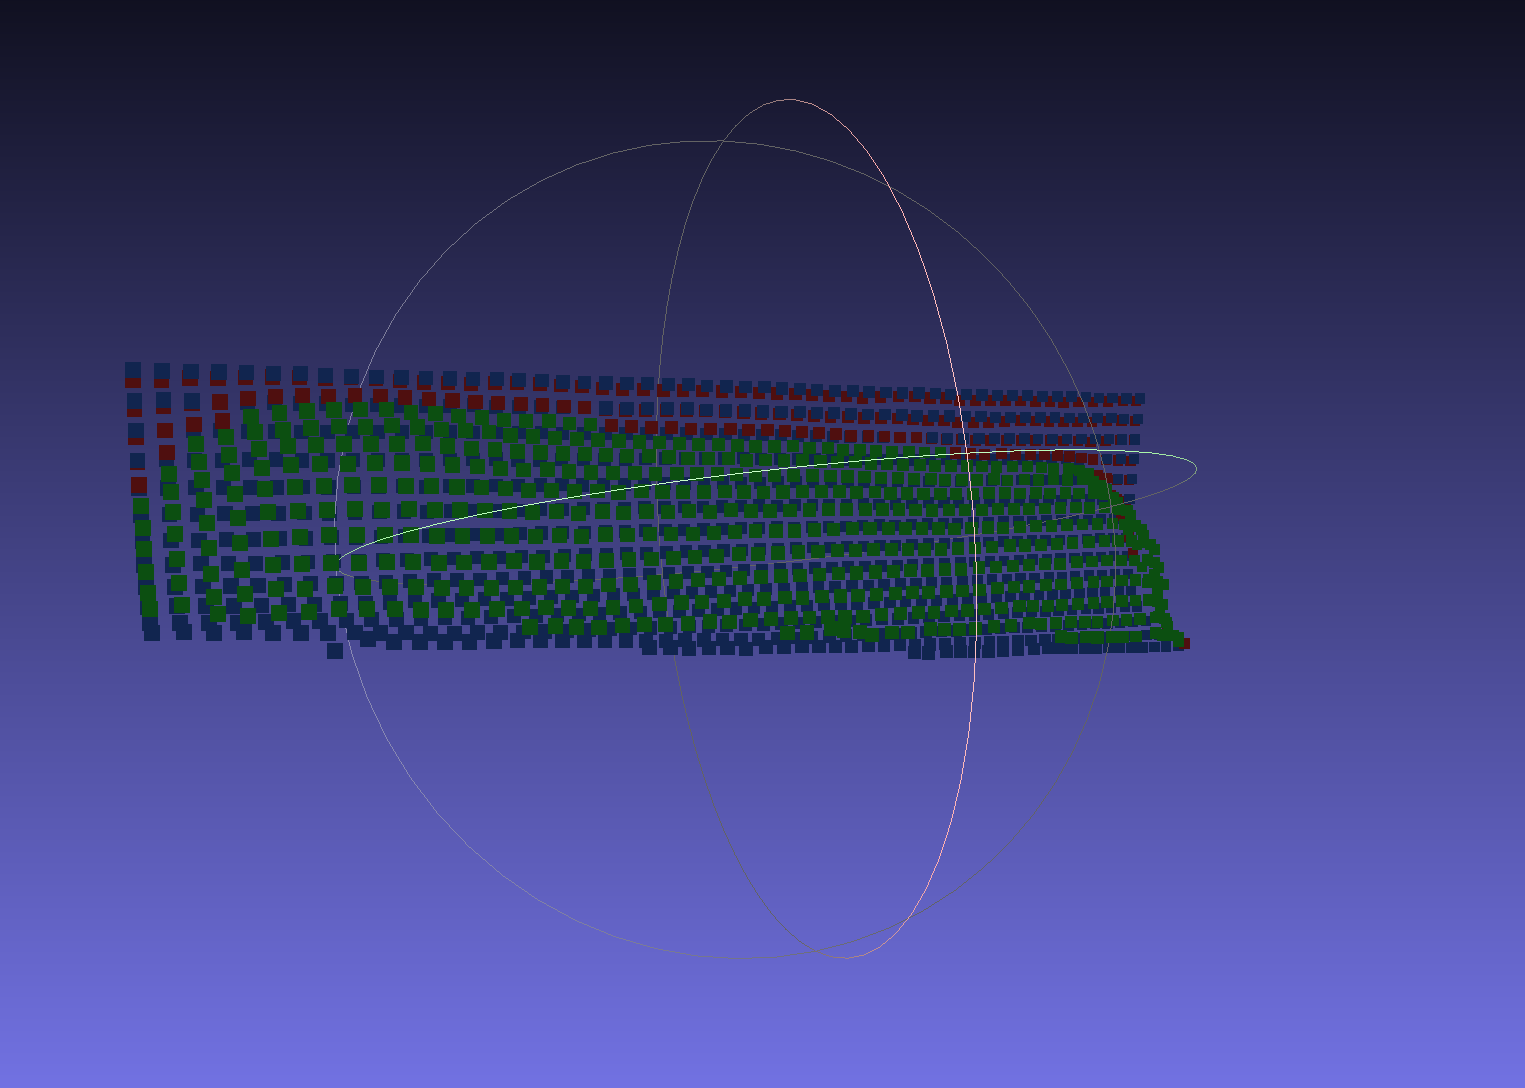
\includegraphics[width=\linewidth]{images/Useful-photos/Screenshots/erosion_front.png}
        \caption{Front view of table-collision filtering}
    \end{subfigure}
    \hfill
    \begin{subfigure}[b]{0.48\textwidth}
        \centering
        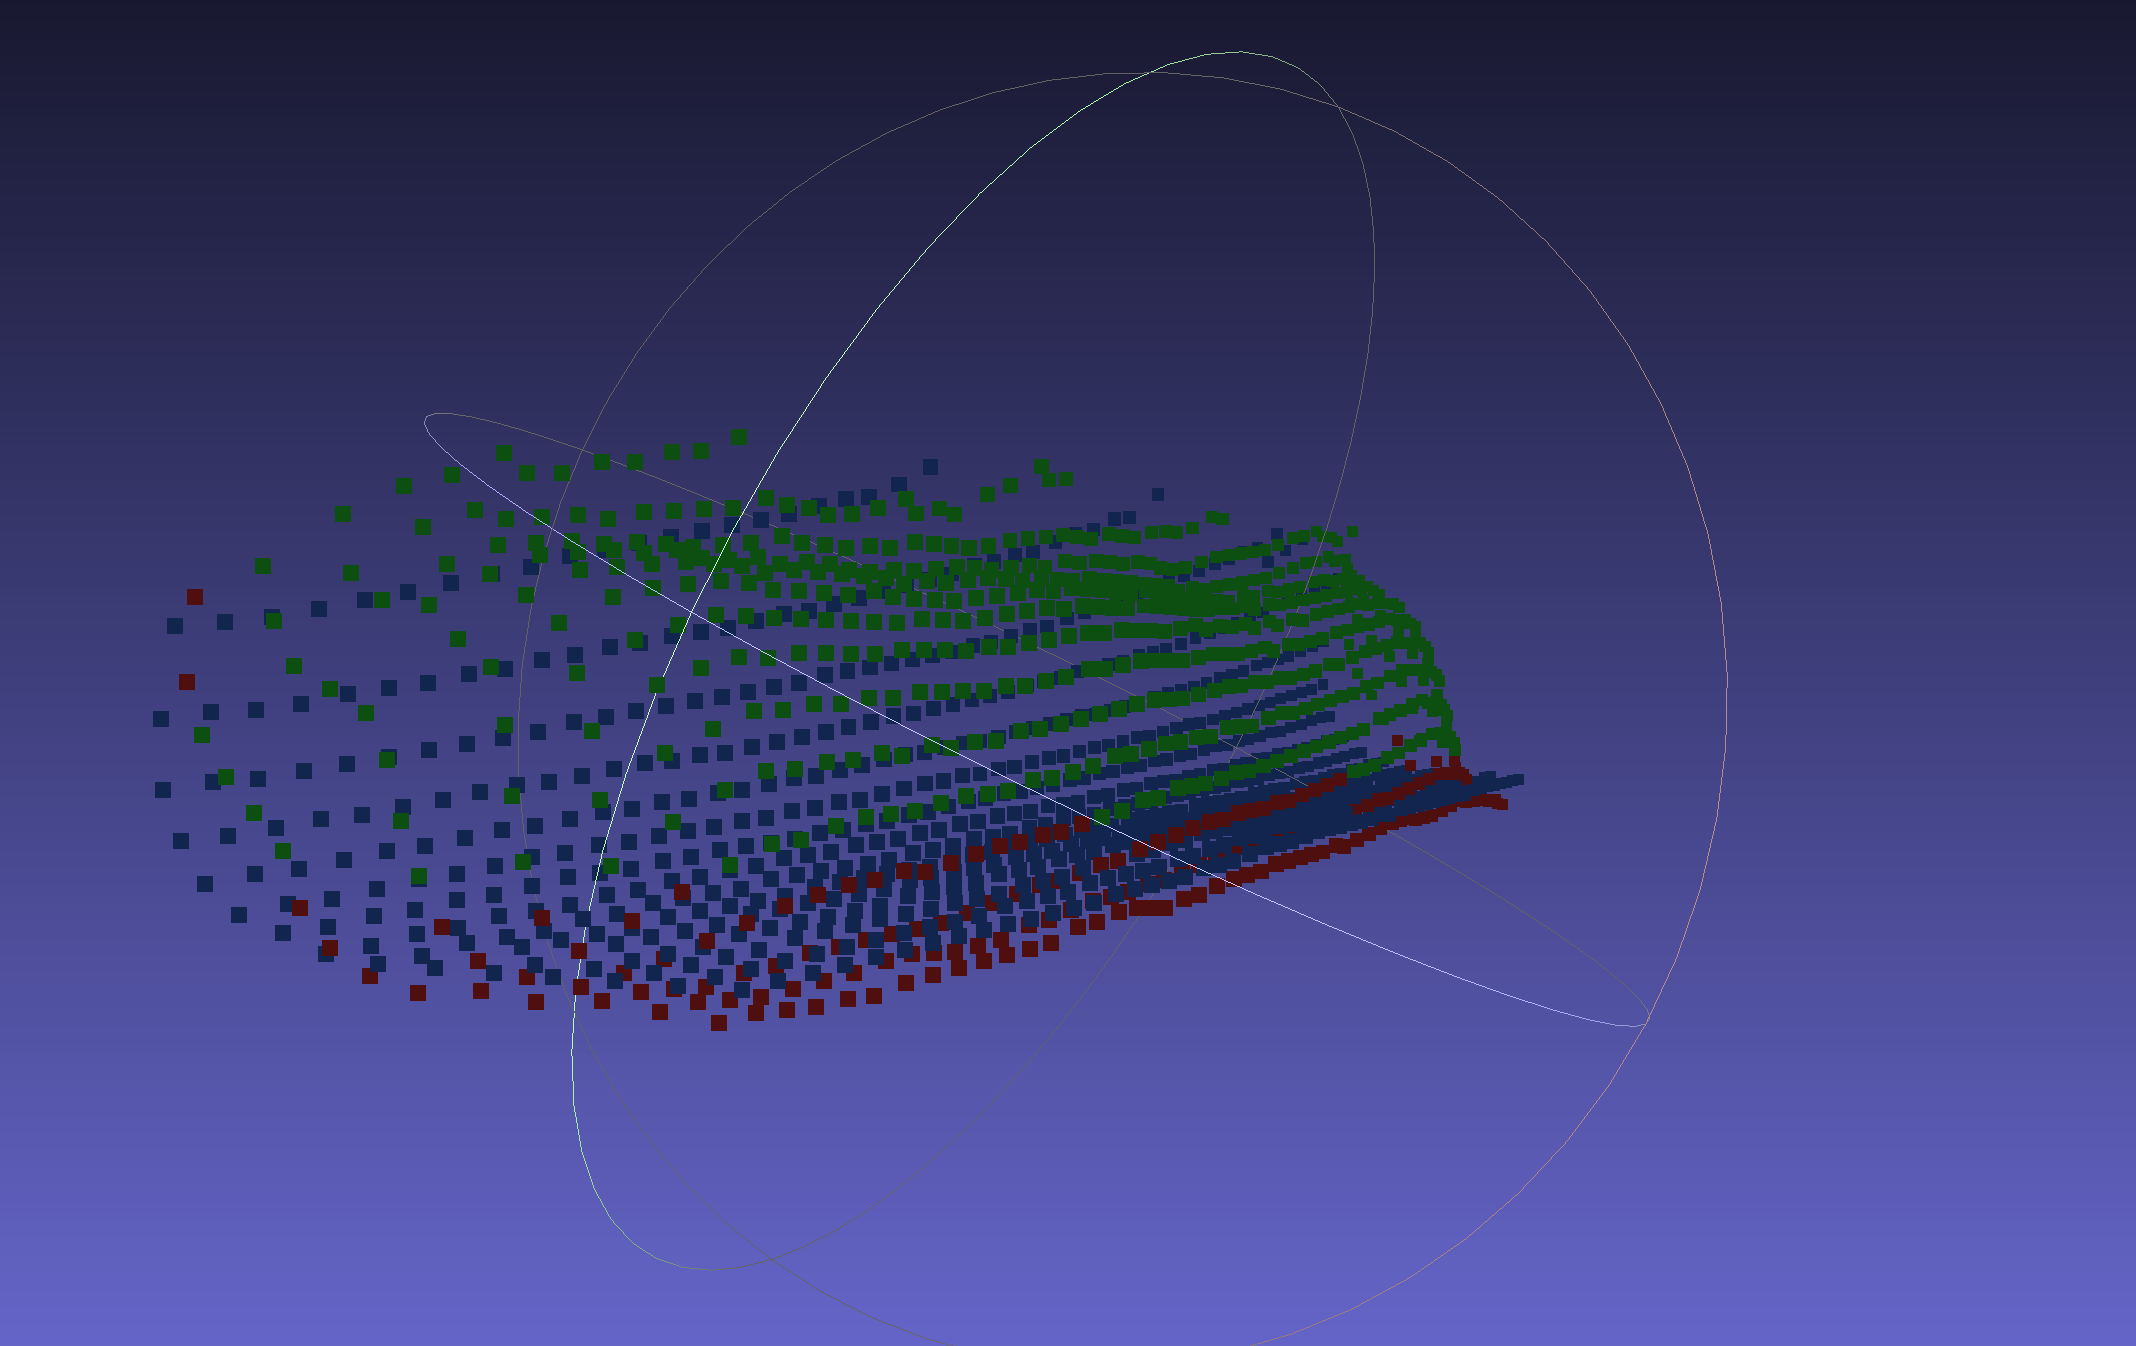
\includegraphics[width=\linewidth]{images/Useful-photos/Screenshots/erosion_side.png}
        \caption{Side view of table-collision filtering}
    \end{subfigure}
    \caption{Examples of depth-based refinement against the reference table model during foreground extraction. Red points are removed because they are too near or intersect the table model (blue points), while the remaining green points are retained as the refined dough foreground.}
\end{figure}

\begin{figure}[H]
    \centering
    \begin{subfigure}[b]{0.48\textwidth}
        \centering
        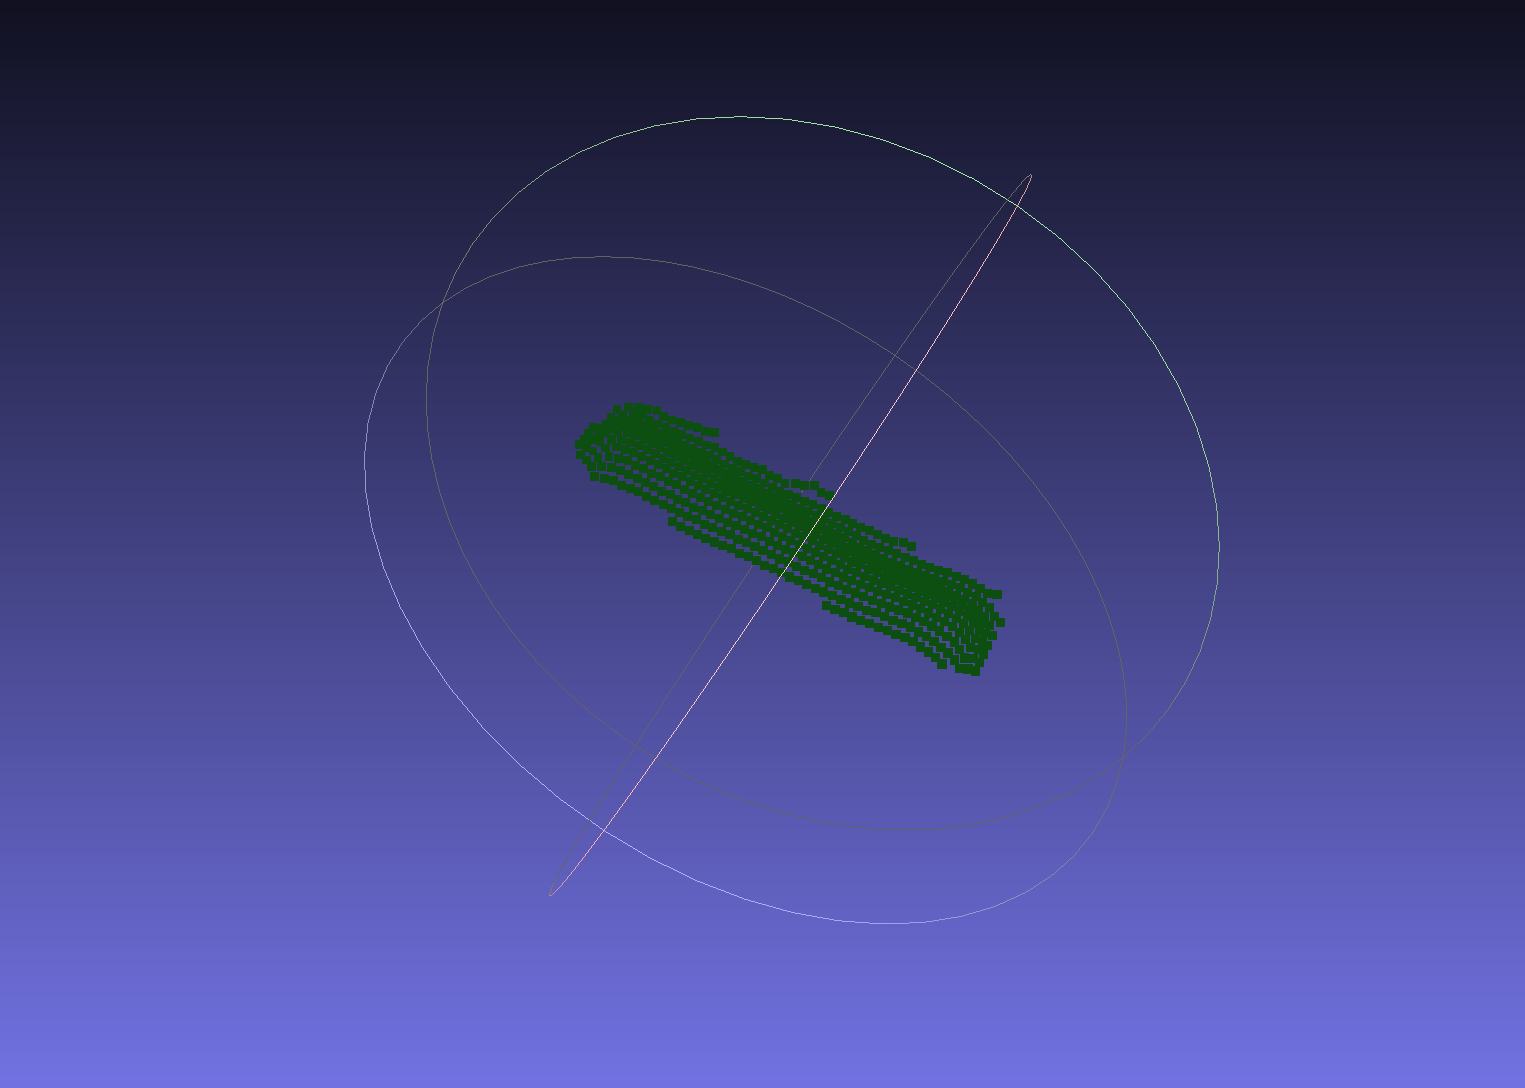
\includegraphics[width=\linewidth]{images/Useful-photos/Screenshots/erosion_result.png}
        \caption{Final foreground after refinement}
    \end{subfigure}
    \hfill
    \begin{subfigure}[b]{0.48\textwidth}
        \centering
        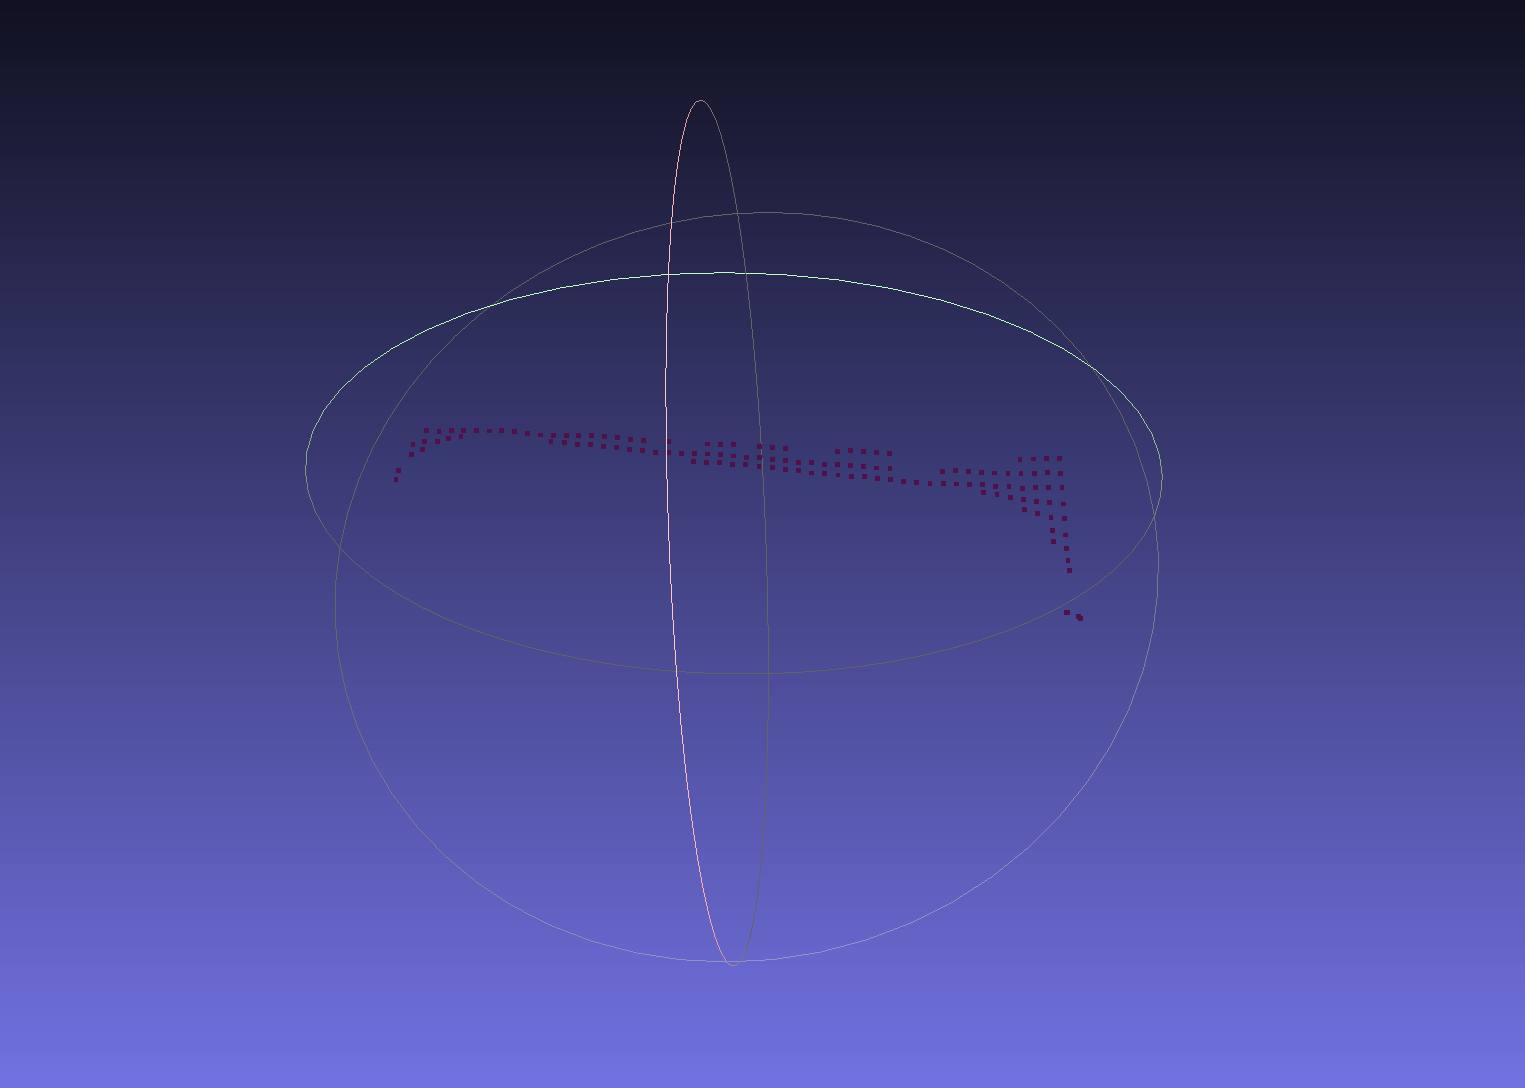
\includegraphics[width=\linewidth]{images/Useful-photos/Screenshots/erosion_removed.png}
        \caption{Points removed during refinement}
    \end{subfigure}
    \caption{Result of the depth-based refinement stage. The left image shows the final foreground after filtering, while the right image highlights the points that were removed because they were inconsistent with the reference table model. This refinement step helps to ensure that the subsequent volume estimation is based on a more accurate representation of the dough geometry.}
    \label{fig:foreground_refinement}
\end{figure}

\subsubsection{Example of Combined Clustering and Background Subtraction}
A representative example of this combined strategy is shown in Figures~\ref{fig:cluster_bgs_input} and~\ref{fig:cluster_bgs_example}. In some cases, the color-clustering stage can include a region that is chromatically similar to the dough but does not belong to the actual product surface. When the corresponding mask is compared with the reference table model, the depth-based background subtraction removes the geometrically inconsistent portion, leaving only the region that is compatible with the dough foreground. This example highlights the practical advantage of combining appearance-based clustering with geometric refinement, since the first stage provides a broad candidate region while the second suppresses portions that are incompatible with the known support geometry.

\begin{figure}[!htbp]
    \centering
    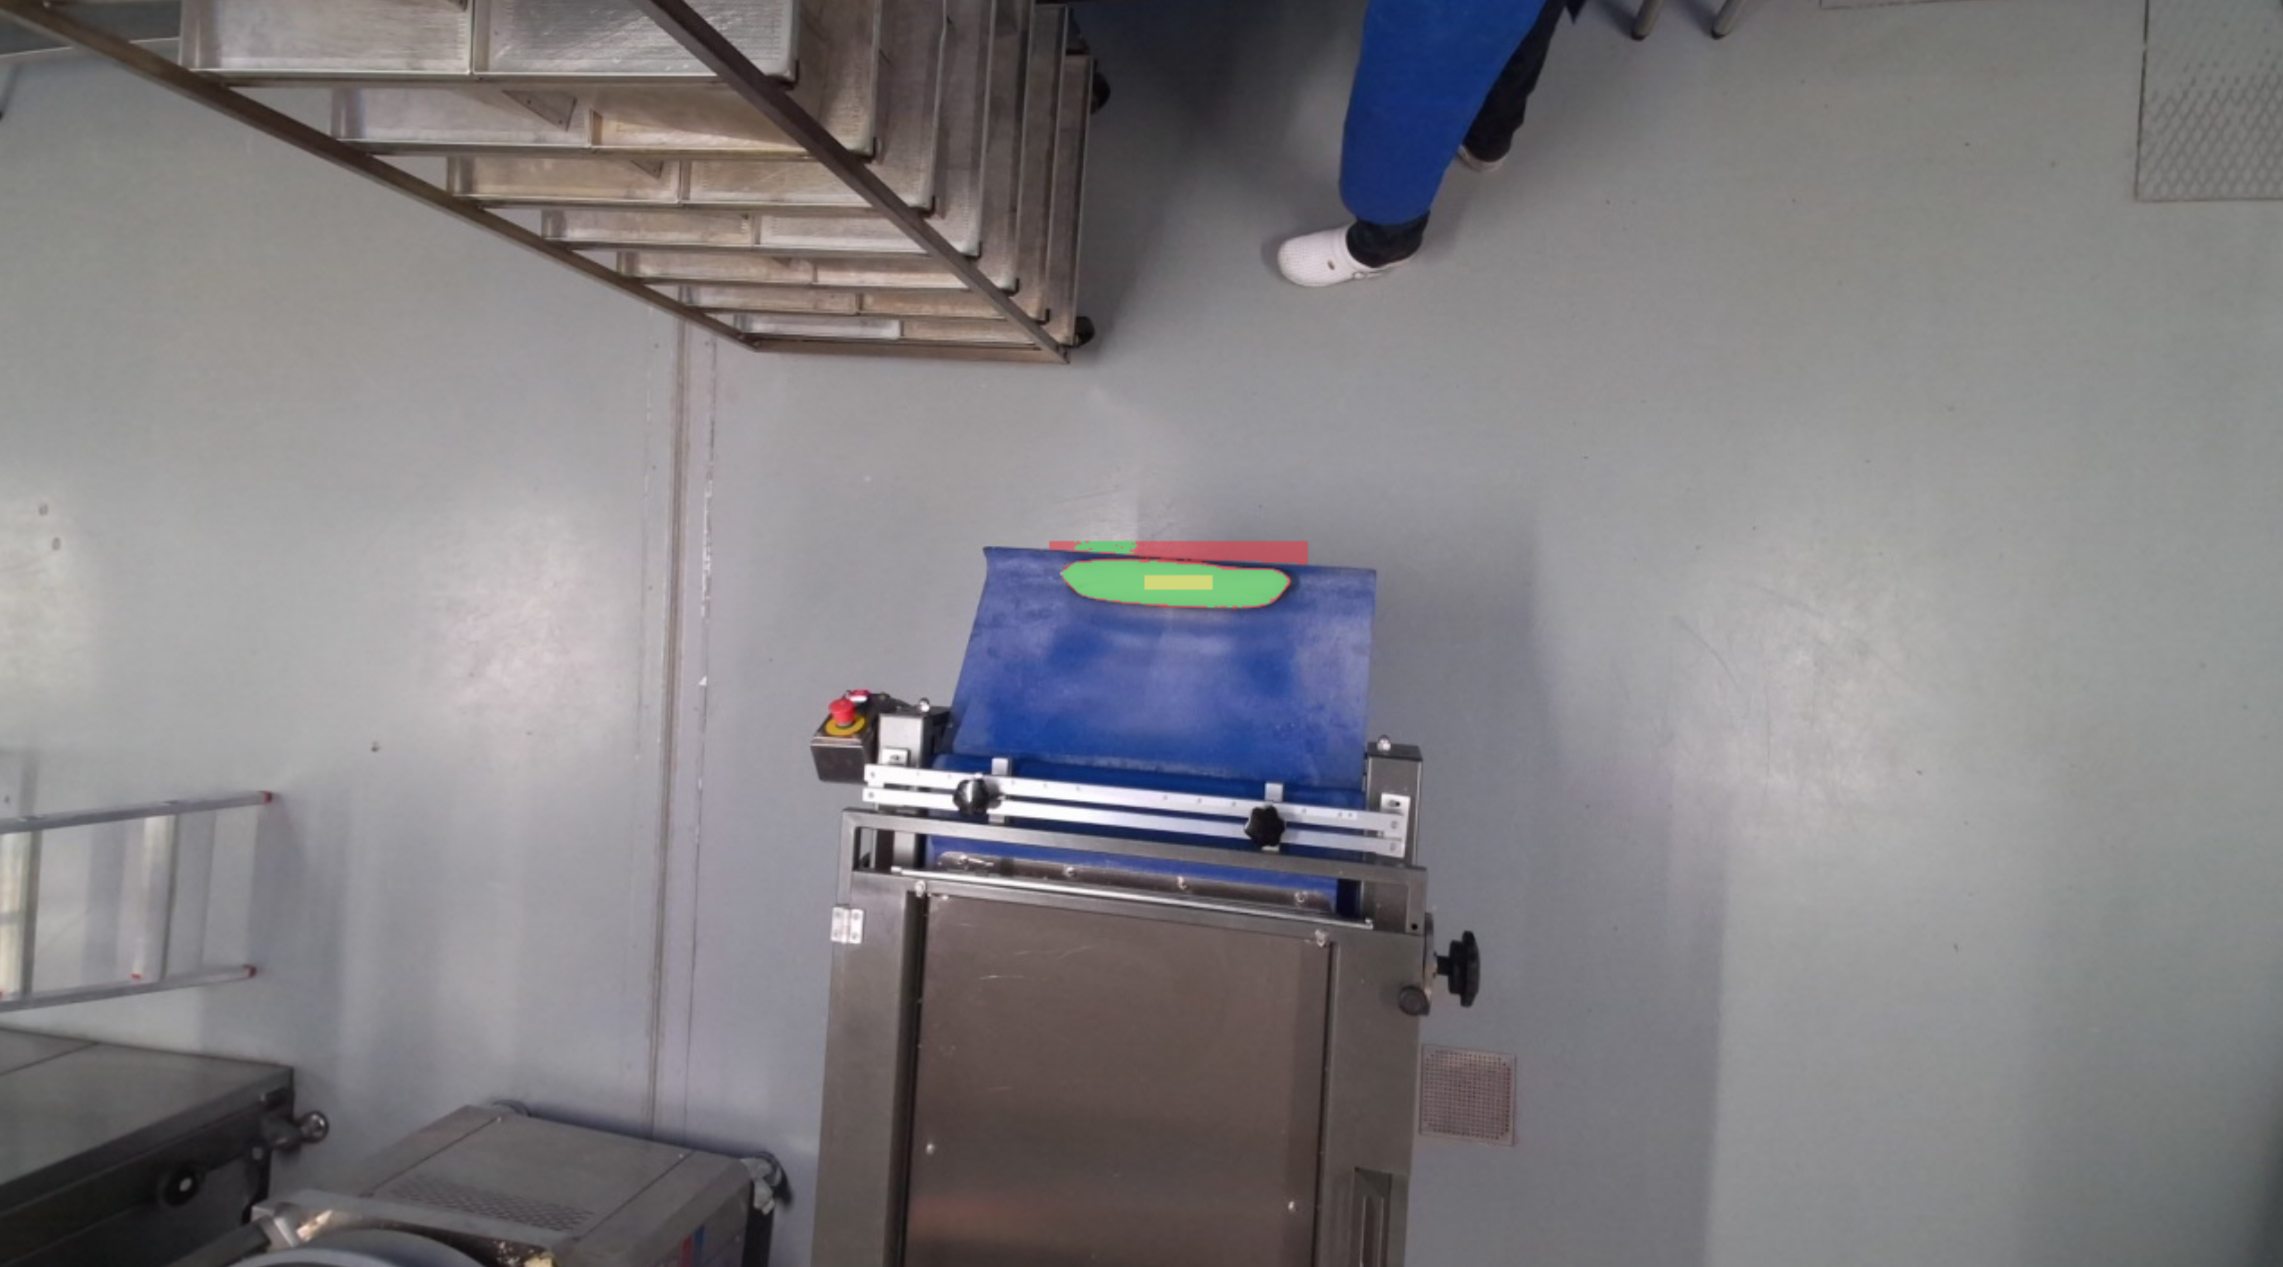
\includegraphics[width=0.58\textwidth]{images/CLuster_1.PNG}
    \caption{Example of bad clustering input. The color-based clustering stage includes an additional region in the upper-left area that is chromatically similar to the dough but does not belong to the actual product surface.}
    \label{fig:cluster_bgs_input}
\end{figure}

\begin{figure}[!htbp]
    \centering
    \begin{subfigure}[t]{0.40\textwidth}
        \centering
        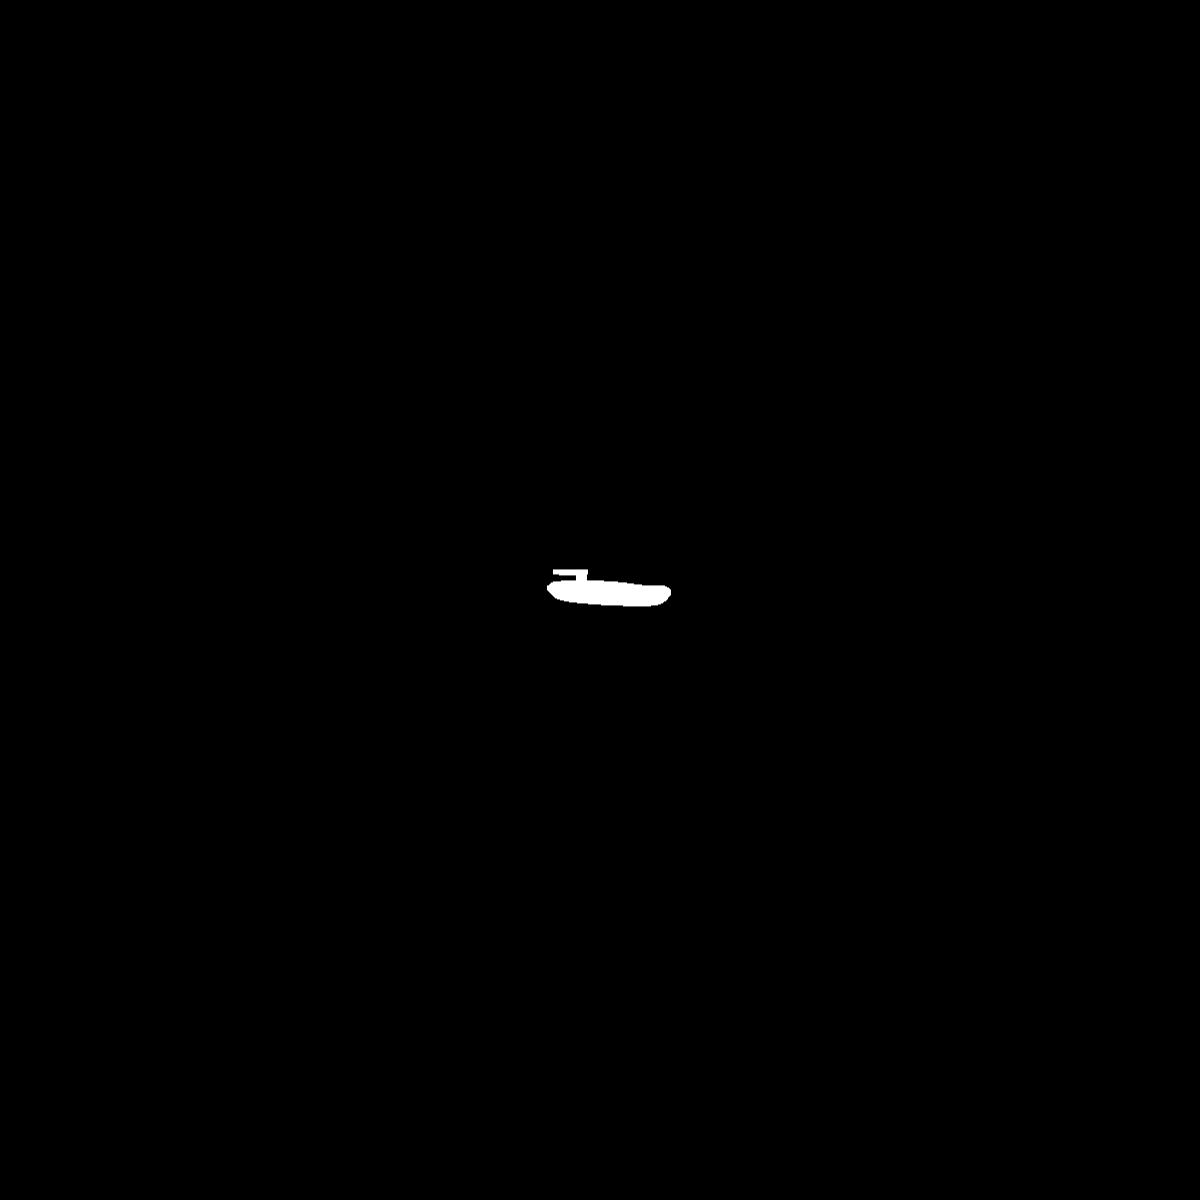
\includegraphics[width=\linewidth]{images/cluster_before.PNG}
        \caption{Mask after color clustering. Note the additional spurious region in the upper-left area}
    \end{subfigure}
    \hfill
    \begin{subfigure}[t]{0.40\textwidth}
        \centering
        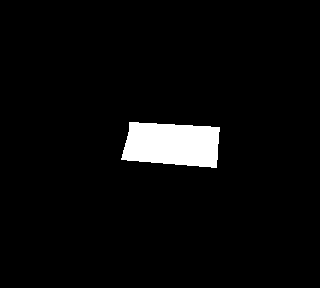
\includegraphics[width=\linewidth]{images/table_bg_table_full_mask.png}
        \caption{Reference table mask}
    \end{subfigure}

    \vspace{0.5em}

    \begin{subfigure}[t]{0.40\textwidth}
        \centering
        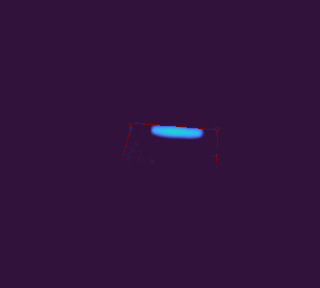
\includegraphics[width=\linewidth]{images/cluster_mid.png}
        \caption{Cluster compared with table model}
    \end{subfigure}
    \hfill
    \begin{subfigure}[t]{0.40\textwidth}
        \centering
        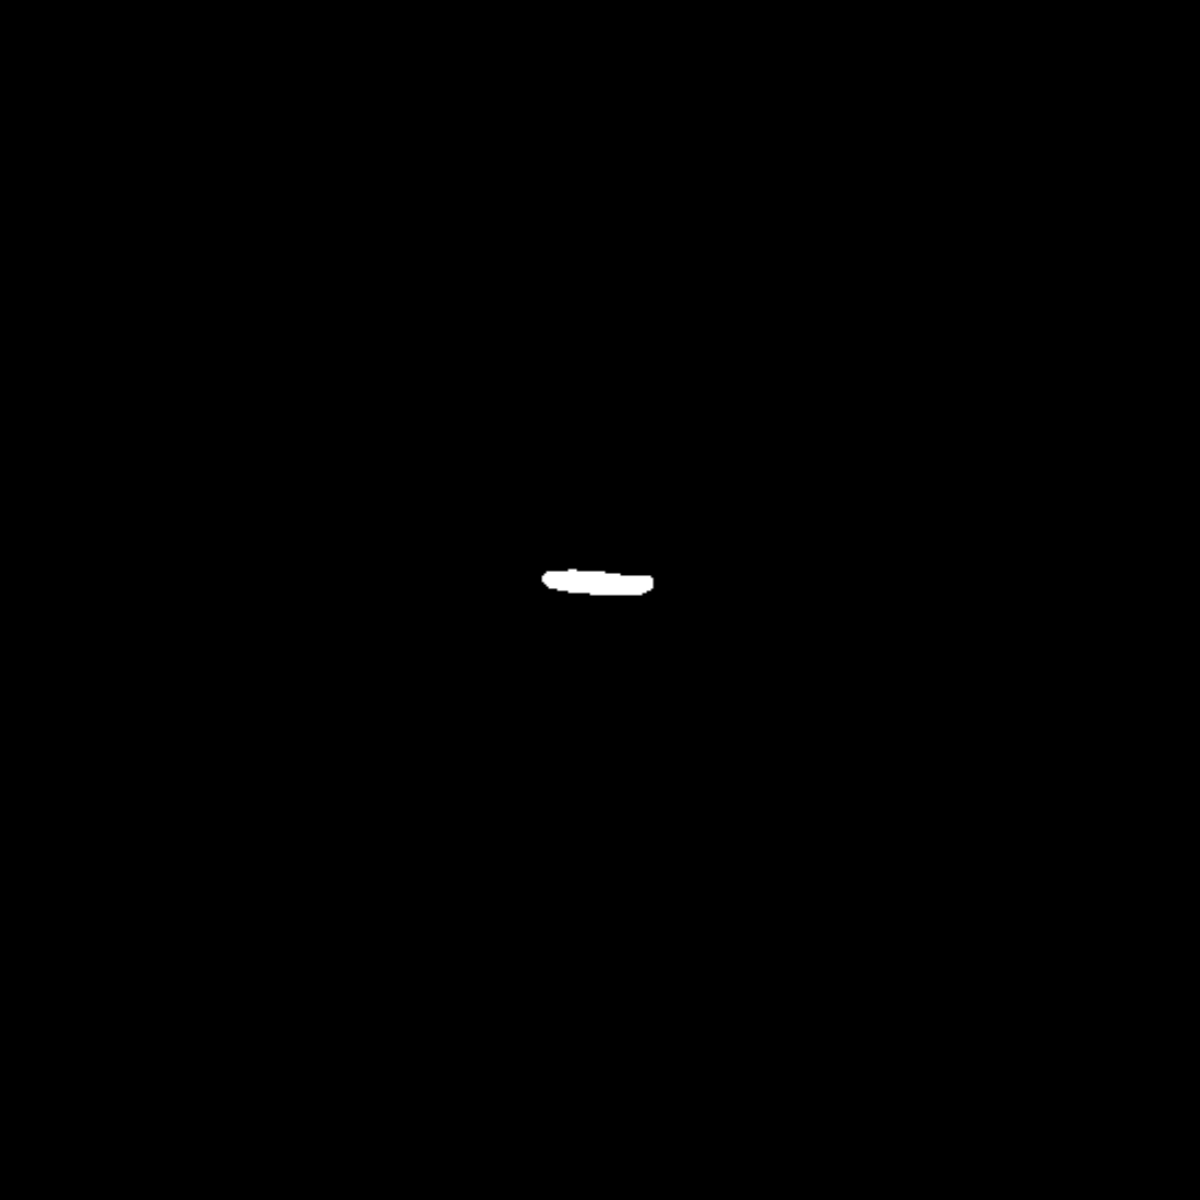
\includegraphics[width=\linewidth]{images/cluster_after.PNG}
        \caption{Final mask after background subtraction}
    \end{subfigure}
    \caption{Example showing the complementarity between color clustering and depth-based background subtraction. The clustering stage initially includes an additional region outside the dough, which is then removed by enforcing consistency with the reference table model.}
    \label{fig:cluster_bgs_example}
\end{figure}
\subsubsection{3D Completion and Volume Estimation}
After foreground extraction, the visible dough points provide only a 2.5D observation of the object. To estimate the hidden lower portion, the implementation supports several completion strategies, including axis-construction modes based on PCA and variants explicitly tied to the support surface.\cite{labby_thesis_repo_2026} In the workflow adopted for the main experiments, the rotated estimators use the \texttt{mid\_support\_pca} strategy: the direction of the rotation axis is derived from PCA on the visible and already filtered dough cloud, while the axis itself is translated so as to lie halfway between the foreground and the support plane. This placement provides a more plausible geometric center for the subsequent rotational completion.

\begin{figure}[H]
    \centering
    \begin{subfigure}[b]{0.48\textwidth}
        \centering
        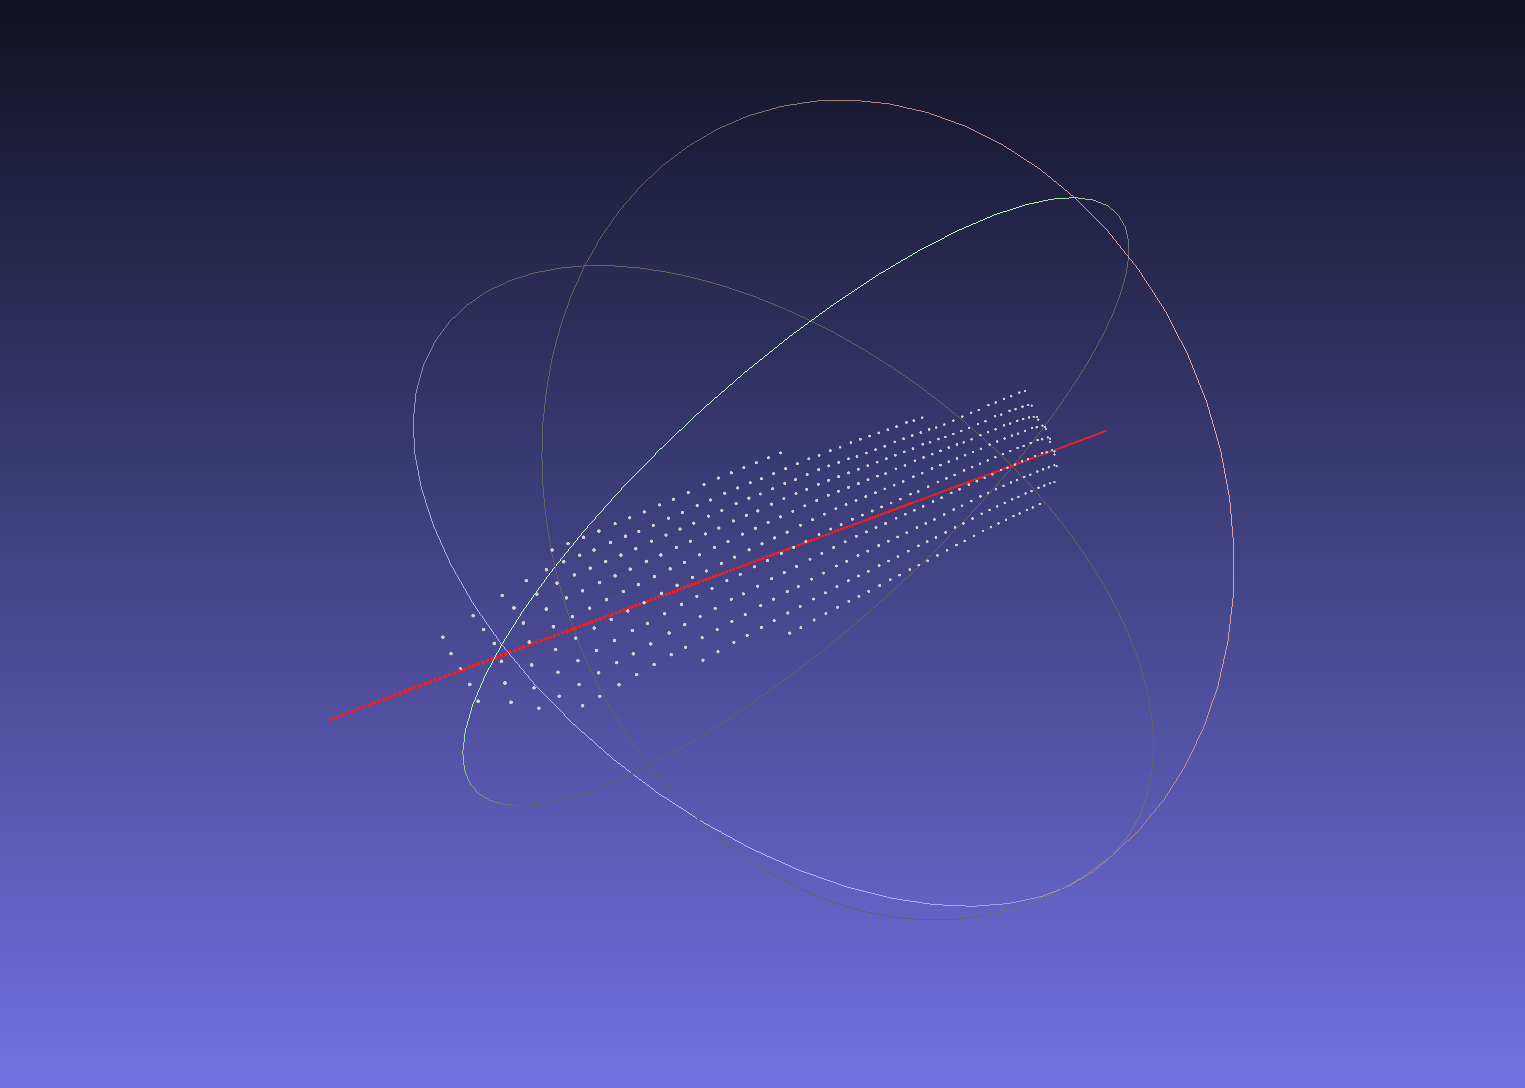
\includegraphics[width=\linewidth]{images/PCA.png}
        \caption{Visible point cloud with rotation axis}
    \end{subfigure}
    \hfill
    \begin{subfigure}[b]{0.48\textwidth}
        \centering
        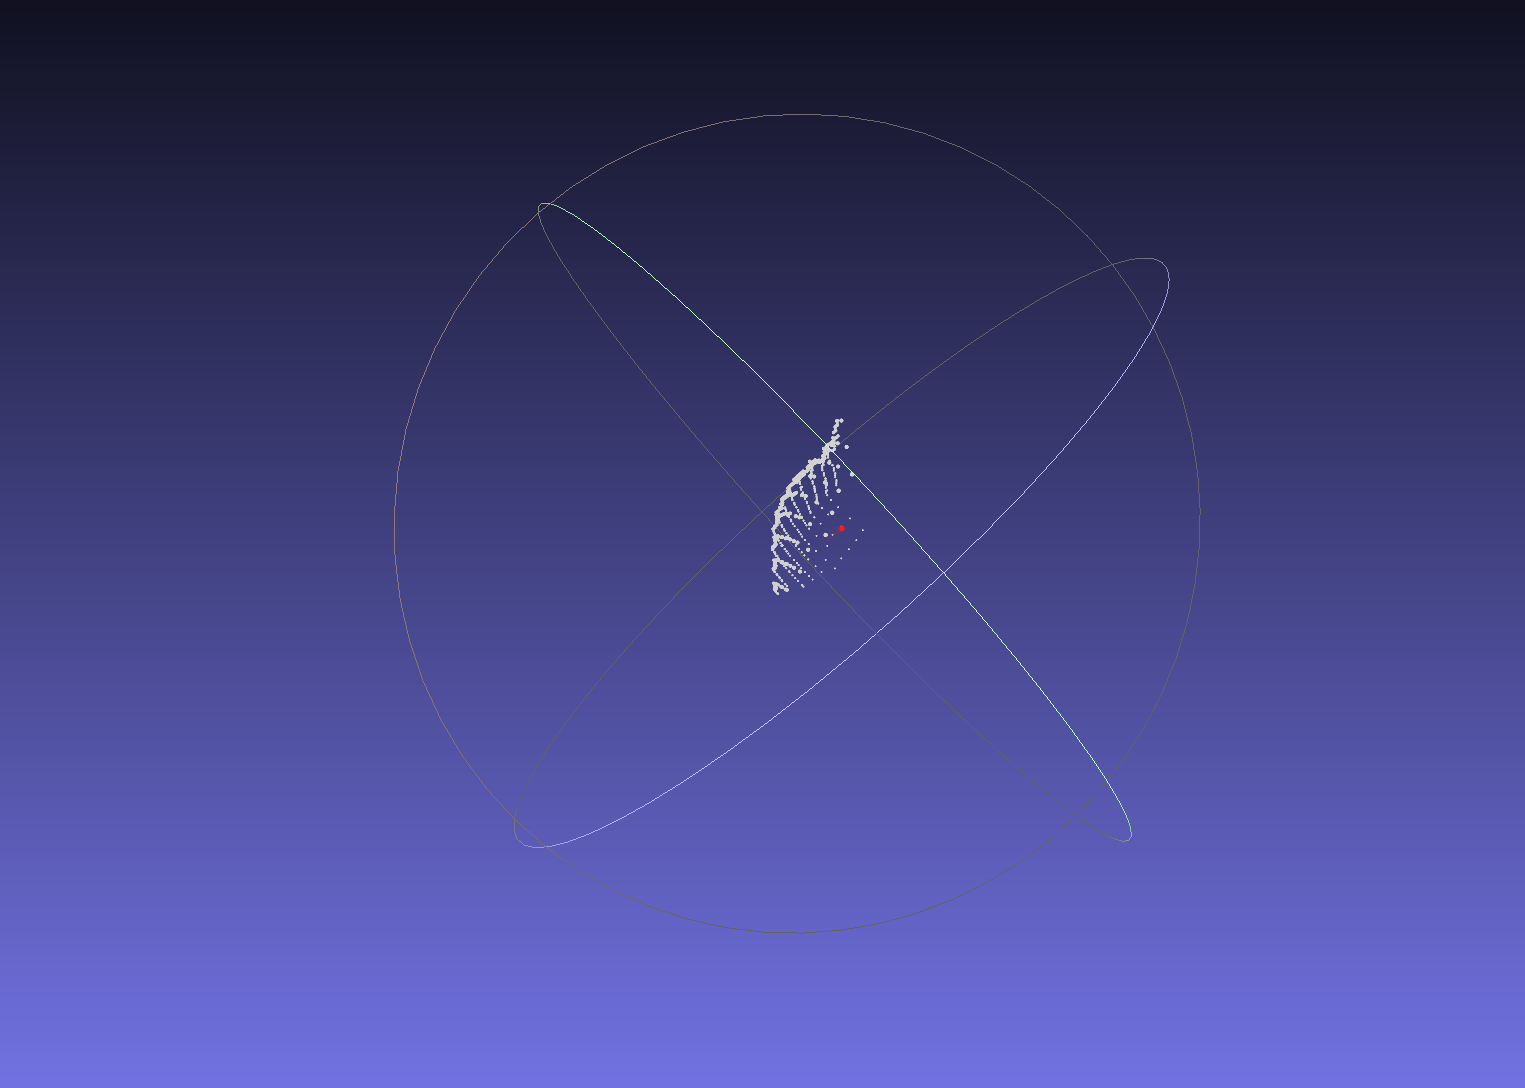
\includegraphics[width=\linewidth]{images/PCA_side.png}
        \caption{Side view of the same configuration}
    \end{subfigure}

    \vspace{0.5em}

    \begin{subfigure}[b]{0.60\textwidth}
        \centering
        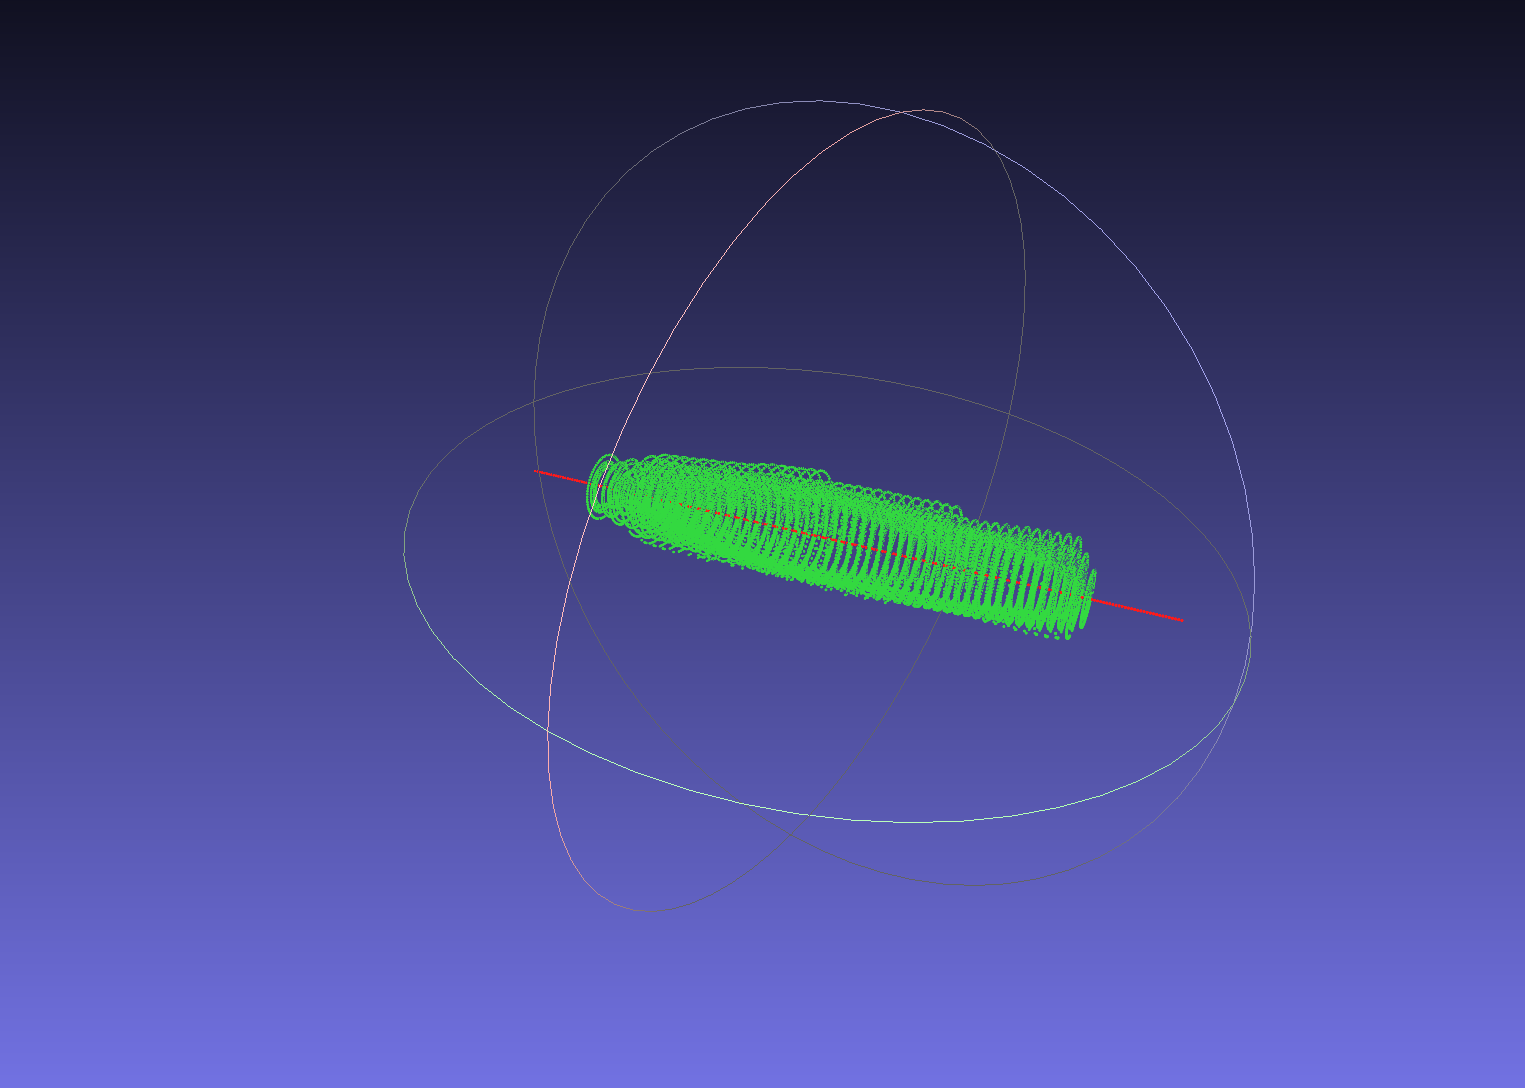
\includegraphics[width=\linewidth]{images/rotated_pc.png}
        \caption{Point cloud after rotational completion}
    \end{subfigure}
    \caption{Example of the geometric completion stage. The first two views show the visible dough point cloud together with the adopted rotation axis (in red), while the third view shows the completed point cloud obtained after rotation.}
    \label{fig:rotation_completion_example}
\end{figure}

The observed geometry is then rotated around this axis, using Rodrigues-based rigid rotations, in order to synthesize an approximation of the non-visible part of the dough. This rotational completion is used only for the rotated convex-hull and rotated alpha-shape estimators. After rotation, points that are geometrically inconsistent with the support model are discarded, and an additional statistical outlier removal stage is applied so that isolated or unstable points do not disproportionately affect the final volume estimate. This cleaning stage is especially important for the rotated estimators, since residual singular depth points near the border of the support can otherwise have a disproportionately large impact when the completion rotates them, leading to a much larger volume estimate.
\\The completed point cloud is then passed to different geometric volume estimators. A raw convex hull computed directly from the visible cloud is used only as an initial baseline and is not retained for the final comparative analysis.

\textbf{Rotated convex hull.} A convex hull is computed after rotational completion of the dough geometry.
\begin{figure}[!htbp]
    \centering
    \begin{subfigure}[b]{0.54\textwidth}
        \centering
        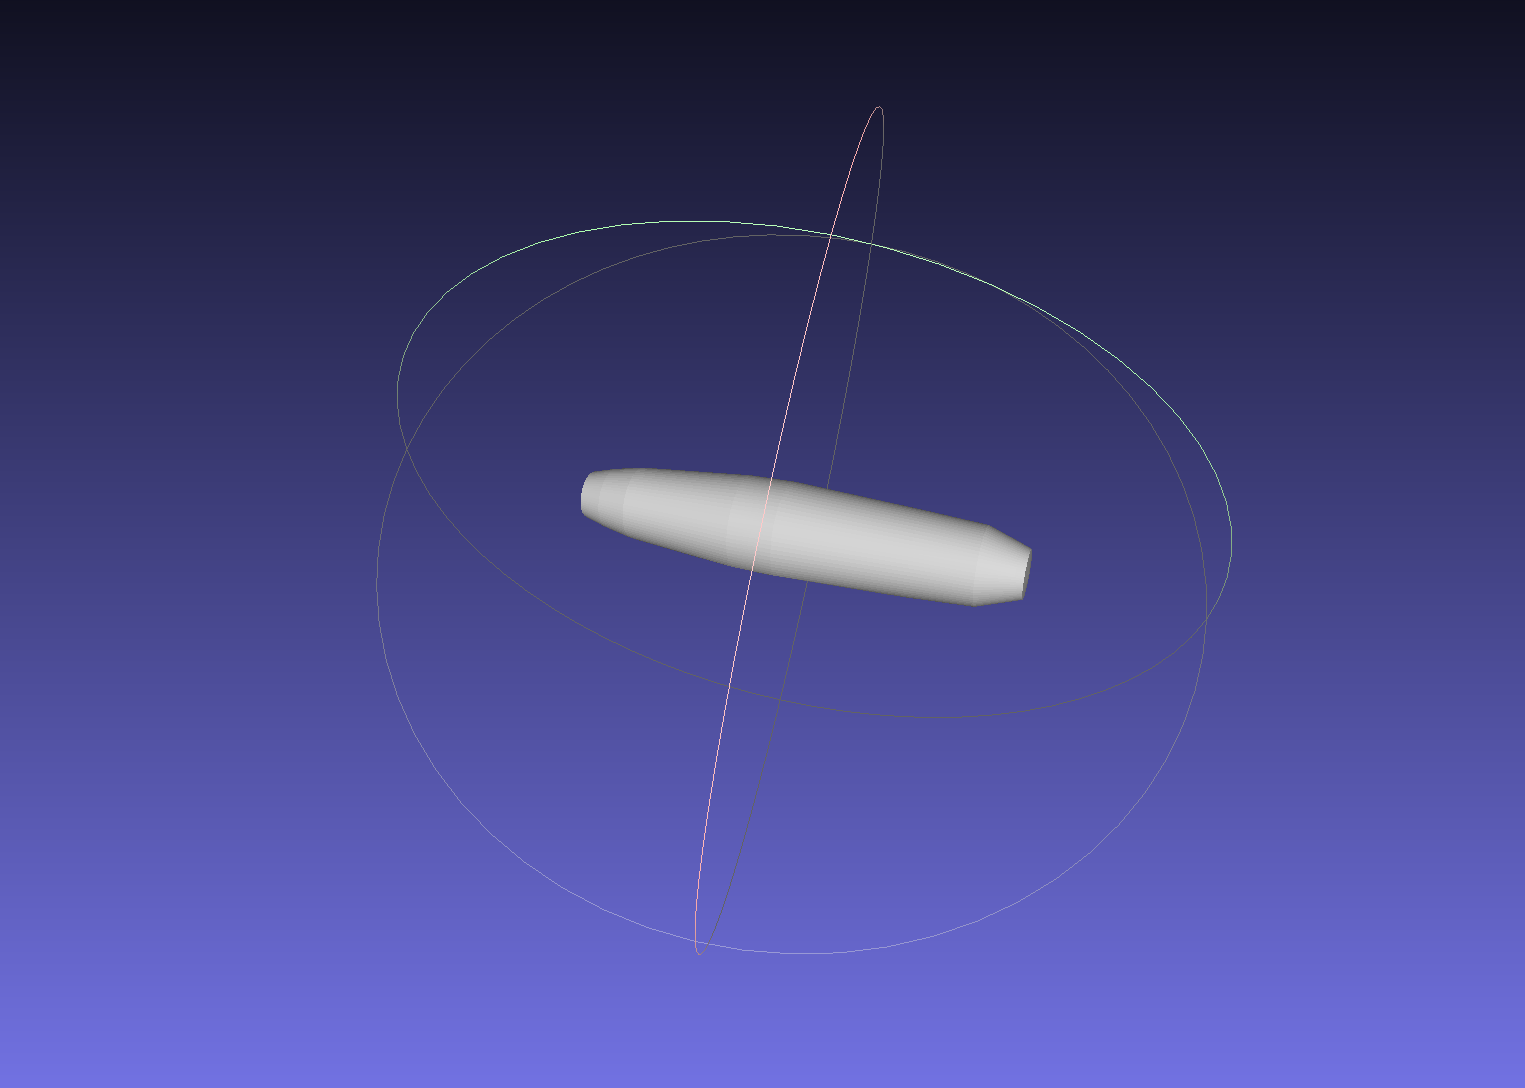
\includegraphics[width=\linewidth]{images/convex.png}
        \caption{Convex-hull mesh}
    \end{subfigure}

    \vspace{0.5em}

    \begin{subfigure}[b]{0.48\textwidth}
        \centering
        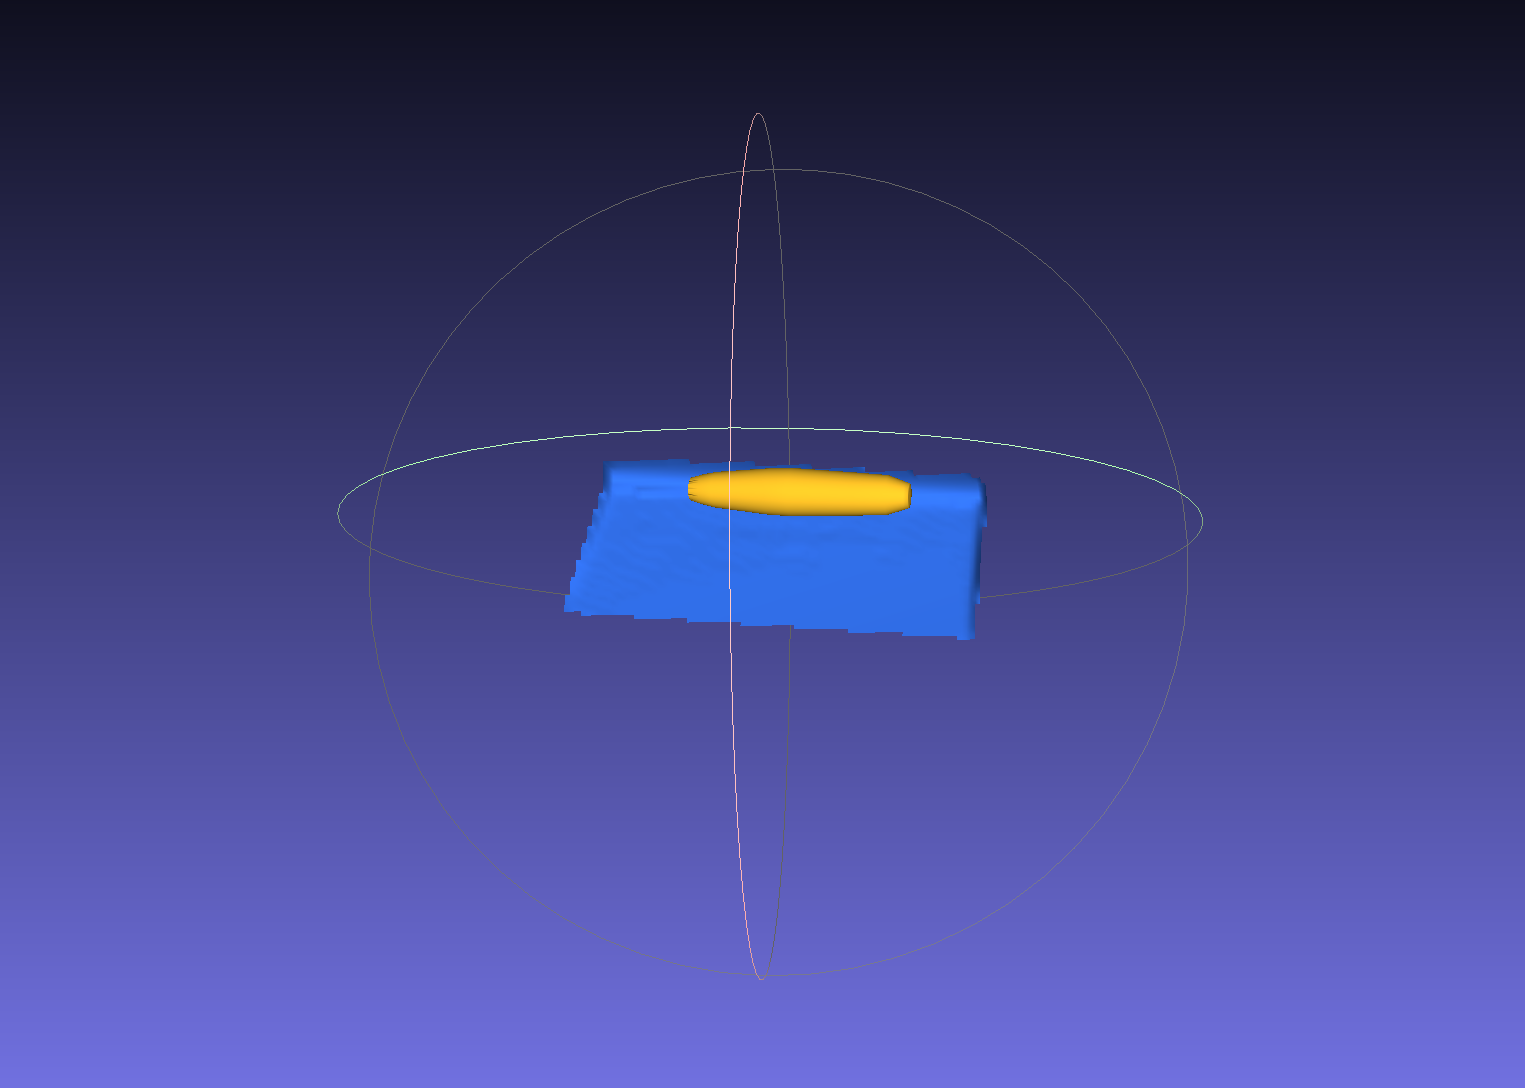
\includegraphics[width=\linewidth]{images/convex_hull_table.png}
        \caption{Front view on the reference table}
    \end{subfigure}
    \hfill
    \begin{subfigure}[b]{0.48\textwidth}
        \centering
        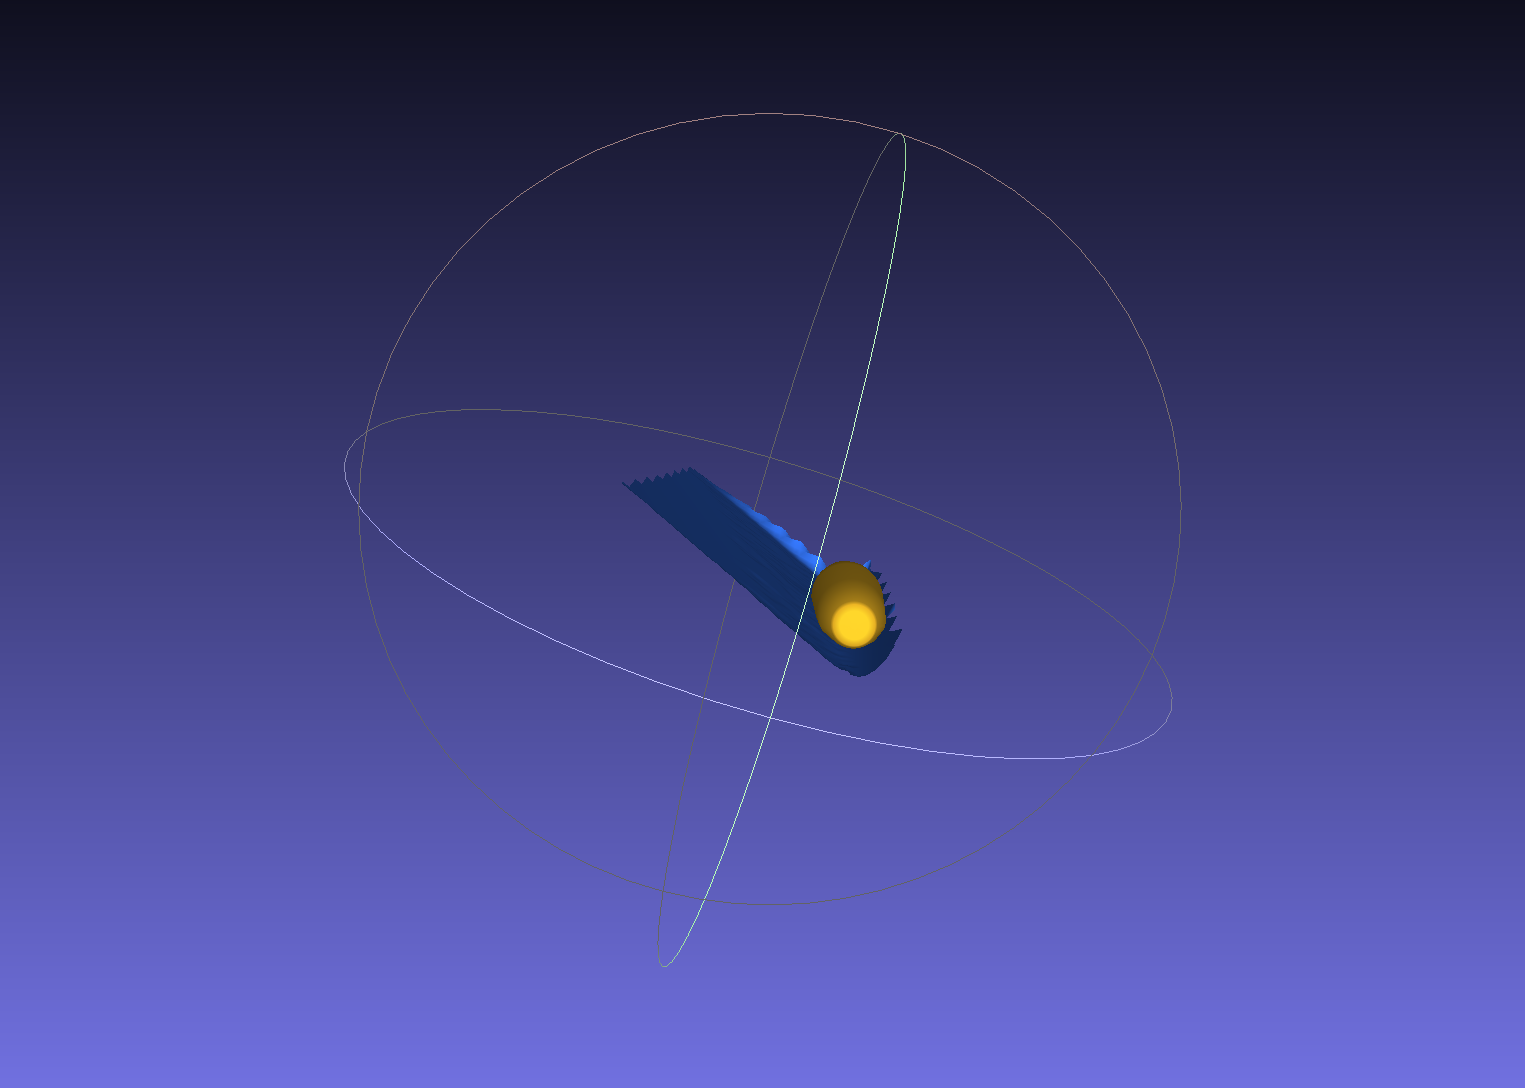
\includegraphics[width=\linewidth]{images/convex_hull_table_side.png}
        \caption{Side view on the reference table}
    \end{subfigure}
    \caption{Representative output of the rotated convex-hull estimator.}
    \label{fig:convex_hull_estimator}
\end{figure}
\newpage
\textbf{Rotated alpha shape.} An alpha-shape reconstruction is computed after rotational completion of the dough geometry.

\begin{figure}[!htbp]
    \centering
    \begin{subfigure}[b]{0.54\textwidth}
        \centering
        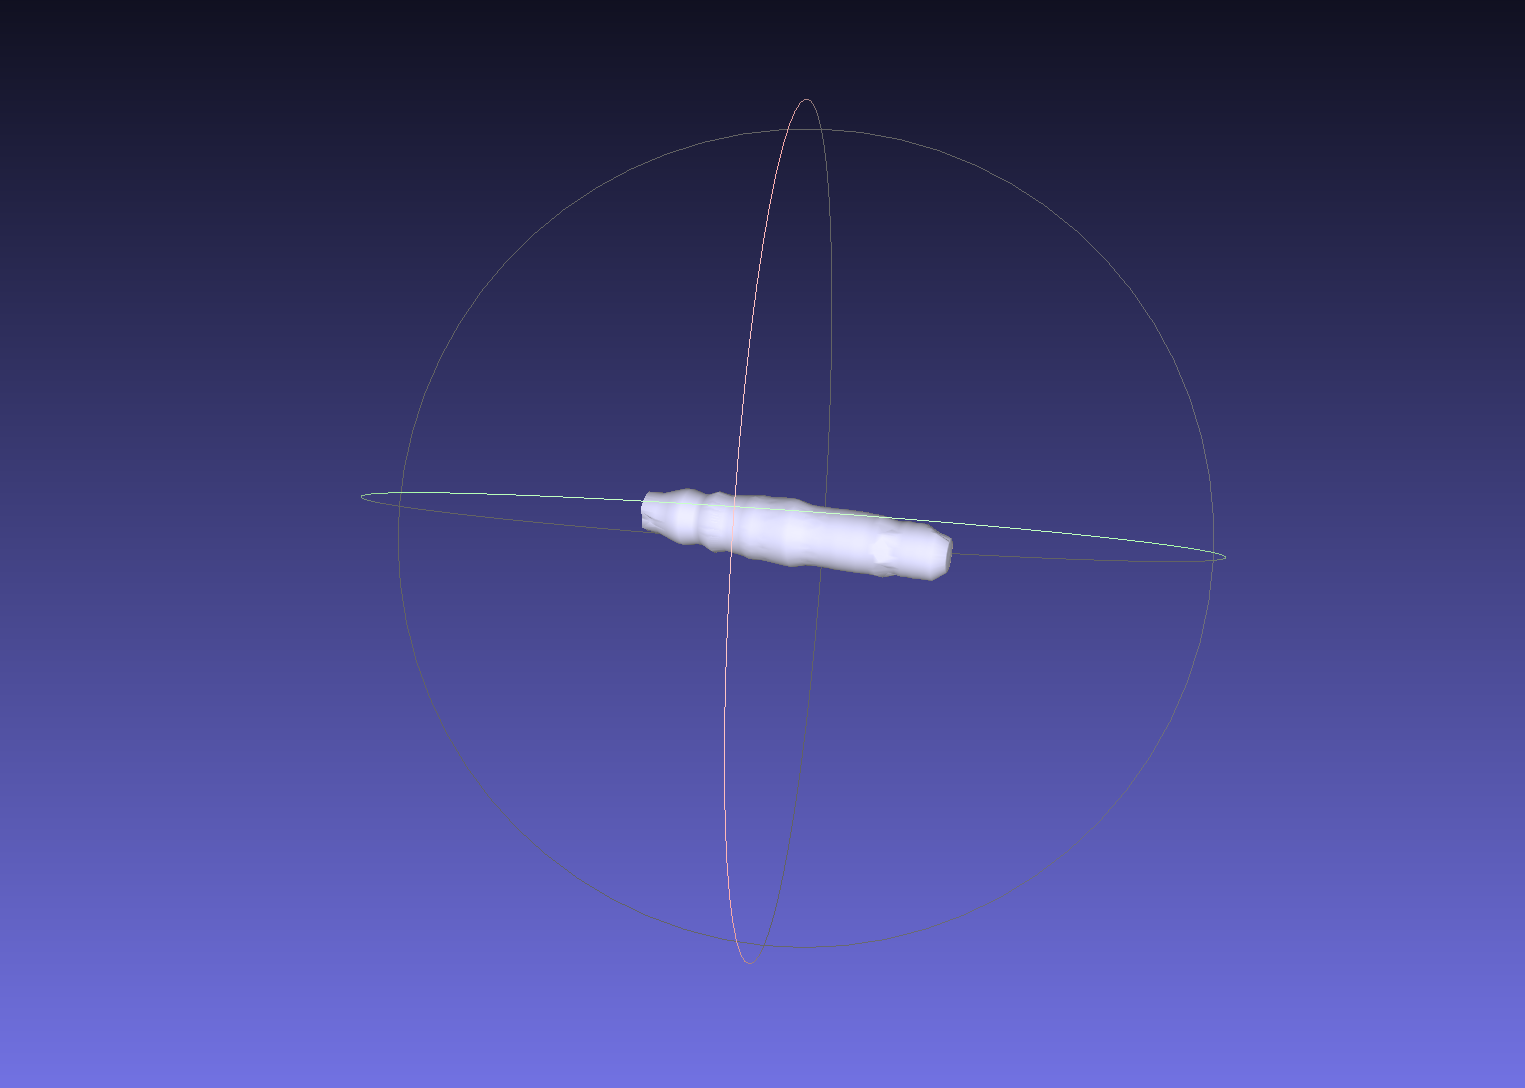
\includegraphics[width=\linewidth]{images/alpha.png}
        \caption{Alpha-shape mesh}
    \end{subfigure}

    \vspace{0.5em}

    \begin{subfigure}[b]{0.48\textwidth}
        \centering
        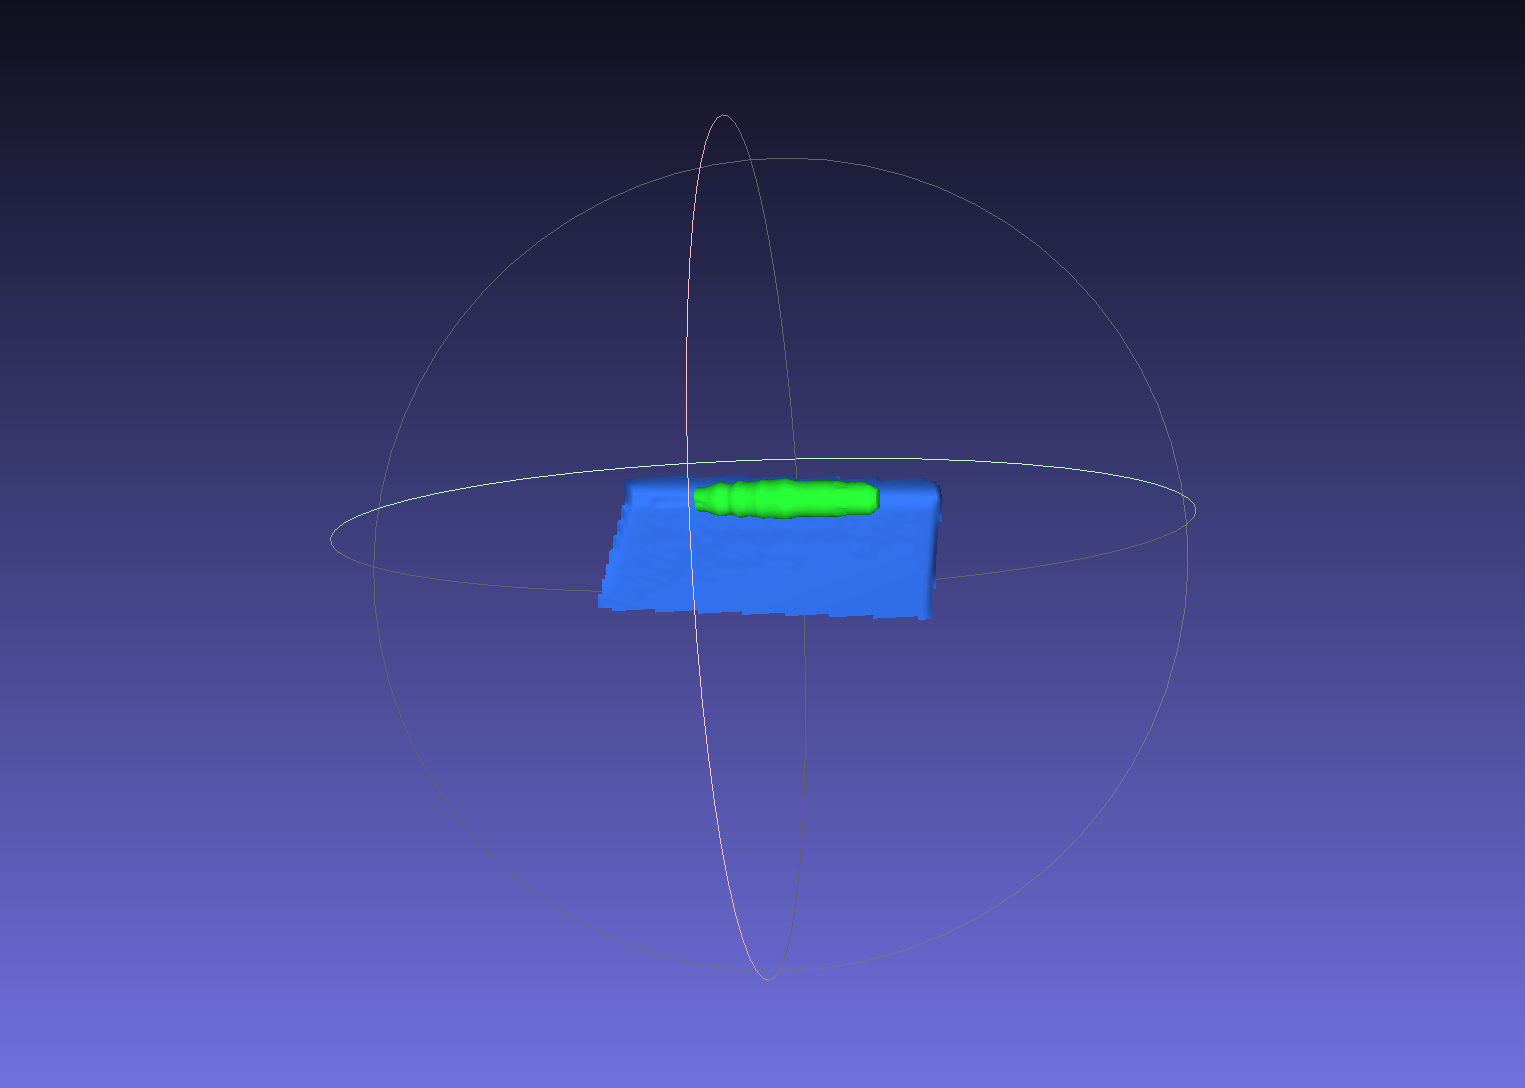
\includegraphics[width=\linewidth]{images/alpha_shape_table.png}
        \caption{Front view on the reference table}
    \end{subfigure}
    \hfill
    \begin{subfigure}[b]{0.48\textwidth}
        \centering
        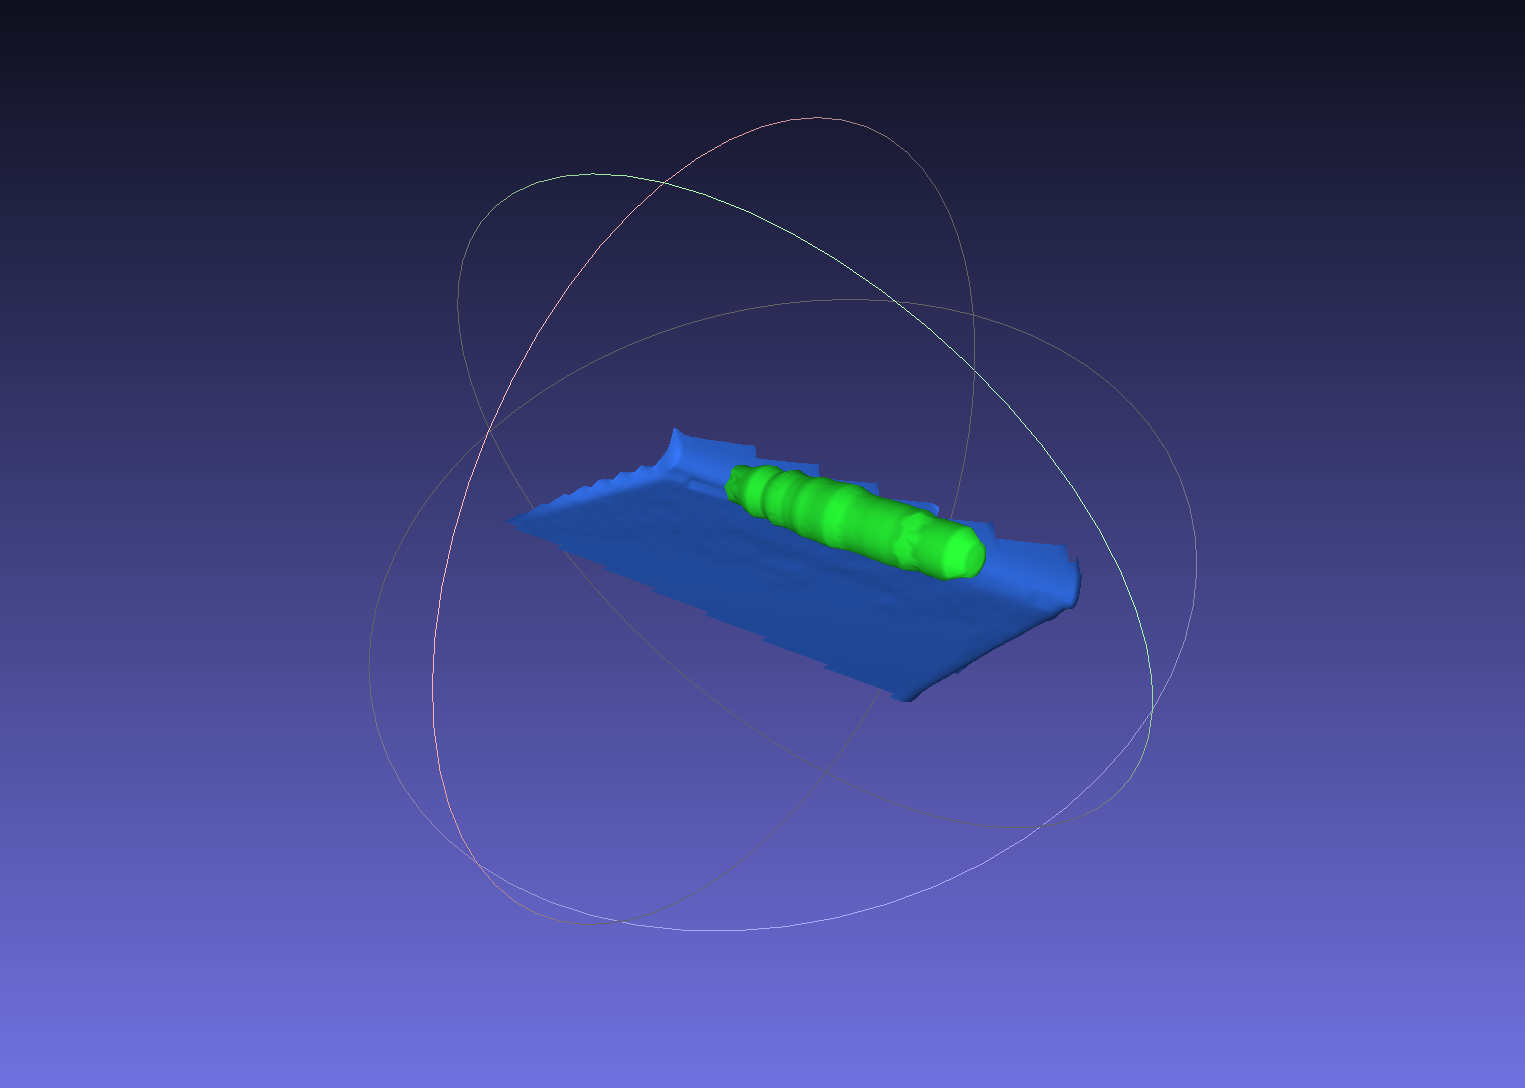
\includegraphics[width=\linewidth]{images/alpha_shape_table_side.png}
        \caption{Side view on the reference table}
    \end{subfigure}
    \caption{Representative output of the rotated alpha-shape estimator.}
    \label{fig:alpha_shape_estimator}
\end{figure}
\newpage
\textbf{Depth-gap estimator.} The \emph{depth-gap} method follows a different logic and does not rely on rotational completion. Instead, it directly fills the space between the segmented foreground and the reference support model.

\begin{figure}[H]
    \centering
    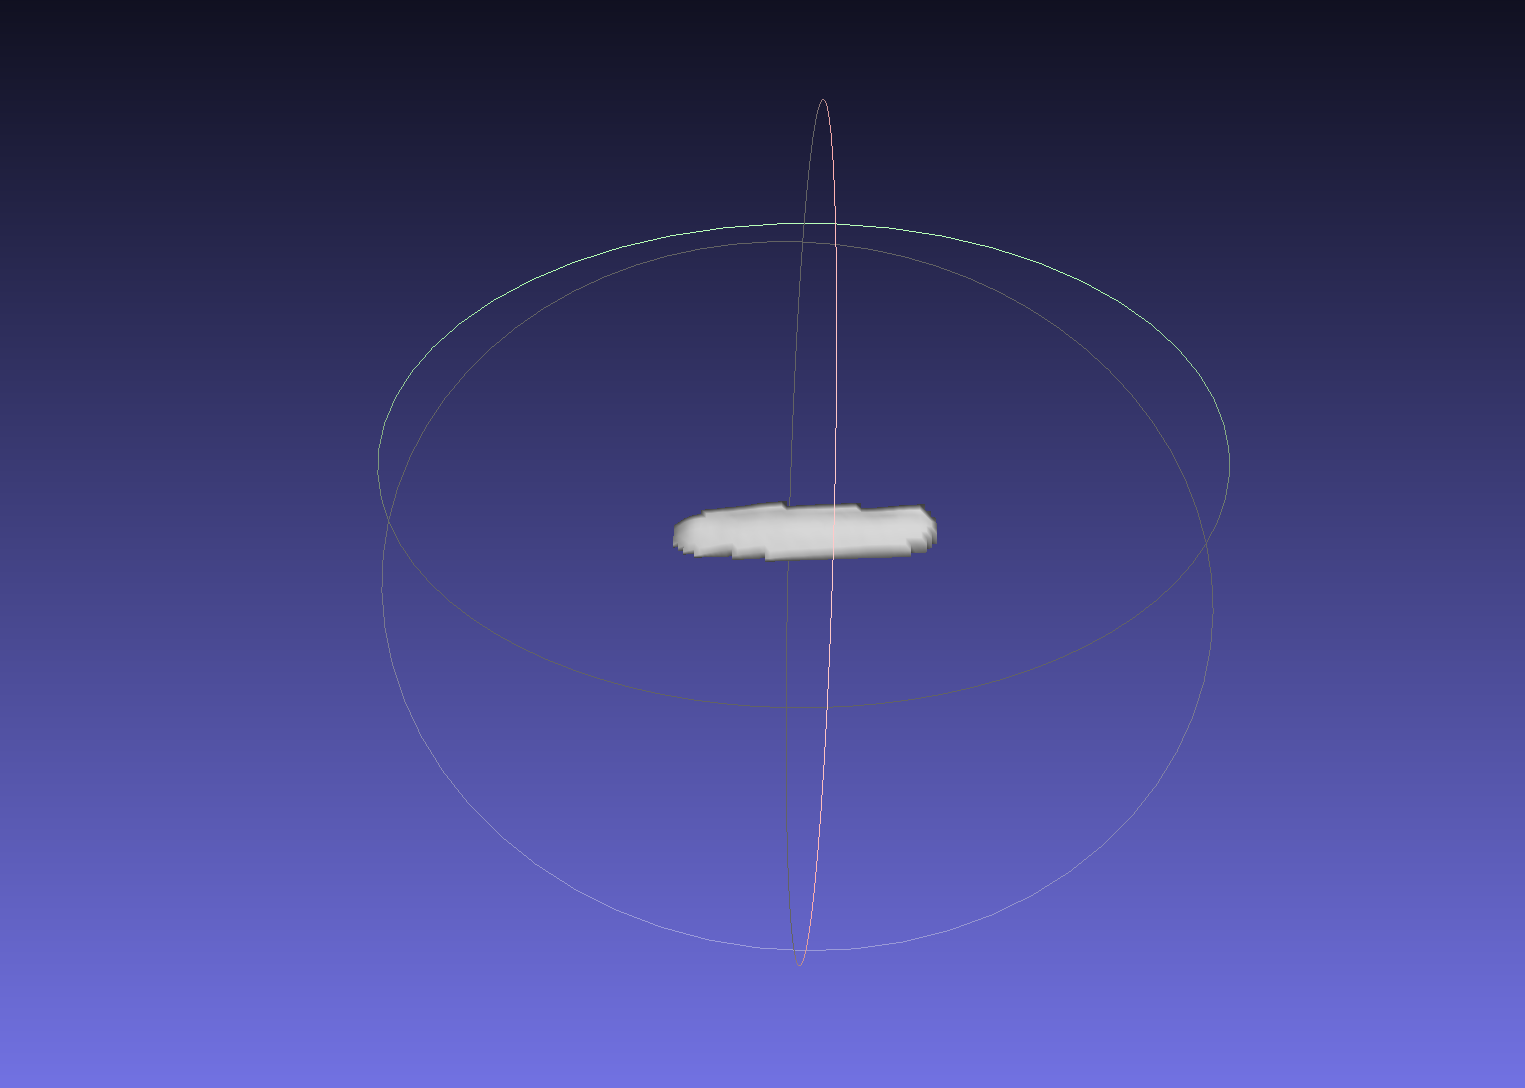
\includegraphics[width=0.70\textwidth]{images/gap.png}
    \caption{Representative output of the \emph{depth-gap} estimator.}
    \label{fig:depth_gap_estimator}
\end{figure}

Representative outputs of the three main estimators considered in this thesis are shown in Figures~\ref{fig:convex_hull_estimator}, \ref{fig:alpha_shape_estimator}, and \ref{fig:depth_gap_estimator}. The full implementation therefore makes it possible to compare simple geometric baselines with progressively more structured reconstructions. In the comparative analysis reported in this thesis, the three main estimators considered over the entire test set are the rotated convex hull, the rotated alpha shape, and the depth-gap method. Their resulting volume distributions are then analyzed and compared in order to assess the consistency of the reconstructed dough volumes, as discussed in Chapter~5.
\newpage
\subsection{Site 2: Anomaly Detection}
At Site~2, the downstream task is not geometric reconstruction but visual anomaly assessment of the final baked product. For this reason, the anomaly-detection branch operates on localized loaf crops rather than on full production-line frames. In the implemented framework, these crops are processed by EfficientAD through anomalib, so that each loaf can be assigned an image-level anomaly score together with spatial diagnostic outputs such as anomaly maps and predicted masks.\cite{batzner_efficientad_2024,akcay_anomalib_2022}

\subsubsection{Dataset Preparation from Loaf Crops}
The first step of the anomaly-detection branch consists of exporting bread-loaf crops from the detector annotations. A dedicated utility reads COCO-style bounding-box annotations, optionally enlarges the crop through configurable padding, discards excessively small detections, and organizes the resulting images into a structure compatible with anomaly-detection training.\cite{labby_thesis_repo_2026}

Two complementary dataset-construction strategies are supported. The first is a simple automatic split, which partitions the crops into train, validation, and test sets according to a 0.8/0.1/0.1 ratio. The second is an interactive review tool through which exported crops can be inspected and manually assigned to good or defective/anomalous subsets before being distributed across the dataset folders.\cite{labby_thesis_repo_2026} This strategy is particularly useful when anomalous samples are few, heterogeneous, externally sourced, or when a small but carefully controlled exploratory dataset is needed. In the present work, this tool was also used in a preliminary test on about 300 good samples, while crops partially occluded by a hand or by the tray were operationally assigned to the defect group. The aim of this test was not to define a representative taxonomy of industrial defects, but to verify whether the network could rapidly separate clearly non-good samples from the good dataset in the event that defective products became available during operation. Since the results of this preliminary test were promising, the model was then trained on the full collected dataset, which was subsequently partitioned into training, validation, and test subsets according to the adopted split.

In the experiments described in this thesis, the normal class is composed of \emph{good} bread images collected during the two-week acquisition campaign. Since no representative defective loaves were provided either by the production site or by the SMACT \cite{smact_official_2026} operators, \textbf{the collected on-site dataset was treated as entirely normal}. To obtain an initial qualitative indication of the model behavior on clearly non-conforming products, a small auxiliary set of \textbf{18 defective bread images} collected \textbf{from online sources} was used as an external reference, with 9 images assigned to the validation set and 9 distinct images assigned to the test set. These images were not used to define the normal training distribution, but only as auxiliary anomalous examples for preliminary qualitative evaluation. They depict clearly non-conforming products, such as burnt or mouldy loaves, but they are not fully representative of either the bread type or the visual environment observed in the industrial setup.

\begin{figure}[H]
    \centering
    \begin{subfigure}[b]{0.24\textwidth}
        \centering
        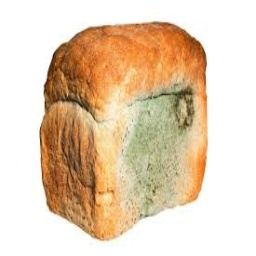
\includegraphics[width=\linewidth]{images/defect1 (1).jpg}
    \end{subfigure}
    \hfill
    \begin{subfigure}[b]{0.24\textwidth}
        \centering
        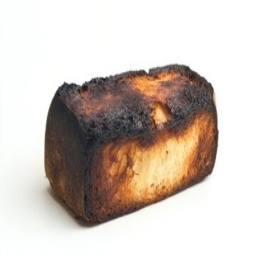
\includegraphics[width=\linewidth]{images/defect1 (2).jpg}
    \end{subfigure}
    \hfill
    \begin{subfigure}[b]{0.24\textwidth}
        \centering
        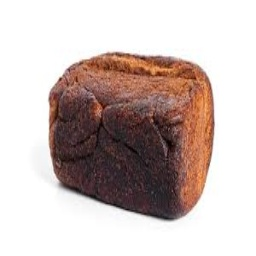
\includegraphics[width=\linewidth]{images/defect1 (3).jpg}
    \end{subfigure}
    \hfill
    \begin{subfigure}[b]{0.24\textwidth}
        \centering
        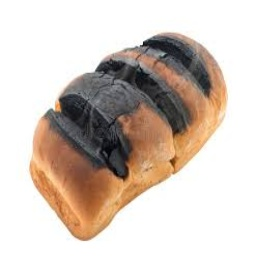
\includegraphics[width=\linewidth]{images/defect1 (4).jpg}
    \end{subfigure}
    \caption{Examples of externally sourced defective bread images used only for qualitative validation and testing of the anomaly-detection branch.}
    \label{fig:site2_external_defects}
\end{figure}

For this reason, they are not expected to provide a rigorous estimate of industrial anomaly-detection performance; rather, they offer a \textbf{practical sanity check} for the anomaly scores and maps produced by the trained model.\cite{labby_thesis_repo_2026} This choice remains consistent with the one-class training paradigm, which focuses on learning the normal class and then relies on anomaly scores to identify deviations from that normality, even when the specific nature of the anomalies is not known in advance.\cite{batzner_efficientad_2024}

\subsubsection{EfficientAD Training}
Once the loaf crops have been organized, EfficientAD is trained through anomalib.\cite{akcay_anomalib_2022} The method remains one-class: it learns the appearance of normal bread from the training set of good samples and later measures deviations from this learned normality at inference time.\cite{batzner_efficientad_2024} Accordingly, the actual training phase is based on the normal samples only, whereas any external anomalous examples are reserved for exploratory validation or qualitative inspection.

The training scripts are designed to be practical for real experimentation. They expose parameters such as image size, batch size, mixed-precision usage, and validation limits, thereby making it possible to adapt the training run to the available GPU memory.\cite{labby_thesis_repo_2026} The implementation also supports scenarios in which anomalous validation or test samples are absent, while still allowing external anomalous images to be included in the validation or test folders whenever a preliminary qualitative check is needed. In this way, the same codebase can be used both for strict one-class training and for exploratory validation of anomaly scores on externally sourced defect examples.

\subsubsection{Inference and Reporting}
After training, the best checkpoint is loaded for inference on batches of loaf crops. Because large inference sets may exceed memory or I/O limits if processed at once, the repository includes a chunked inference routine that iterates over the dataset in manageable groups and stores the predictions incrementally.\cite{labby_thesis_repo_2026}

For each analyzed crop, the implemented pipeline produces an image-level anomaly score, a predicted class label, an anomaly map, and a binary mask. The outputs are then saved both in numerical form, through CSV and text summaries, and in visual form, through heatmaps, overlays, and dedicated debug folders containing the most anomalous examples.\cite{labby_thesis_repo_2026} In the context of this thesis, the most relevant quantity is the anomaly score itself, since it provides the scalar measure used to compare samples and to analyze the distribution of potentially problematic loaves over the inspected set.
These results are then shown and analyzed in Chapter~5.
